% Options for packages loaded elsewhere
\PassOptionsToPackage{unicode}{hyperref}
\PassOptionsToPackage{hyphens}{url}
%
\documentclass[
]{article}
\usepackage{lmodern}
\usepackage{amssymb,amsmath}
\usepackage{ifxetex,ifluatex}
\ifnum 0\ifxetex 1\fi\ifluatex 1\fi=0 % if pdftex
  \usepackage[T1]{fontenc}
  \usepackage[utf8]{inputenc}
  \usepackage{textcomp} % provide euro and other symbols
\else % if luatex or xetex
  \usepackage{unicode-math}
  \defaultfontfeatures{Scale=MatchLowercase}
  \defaultfontfeatures[\rmfamily]{Ligatures=TeX,Scale=1}
\fi
% Use upquote if available, for straight quotes in verbatim environments
\IfFileExists{upquote.sty}{\usepackage{upquote}}{}
\IfFileExists{microtype.sty}{% use microtype if available
  \usepackage[]{microtype}
  \UseMicrotypeSet[protrusion]{basicmath} % disable protrusion for tt fonts
}{}
\makeatletter
\@ifundefined{KOMAClassName}{% if non-KOMA class
  \IfFileExists{parskip.sty}{%
    \usepackage{parskip}
  }{% else
    \setlength{\parindent}{0pt}
    \setlength{\parskip}{6pt plus 2pt minus 1pt}}
}{% if KOMA class
  \KOMAoptions{parskip=half}}
\makeatother
\usepackage{xcolor}
\IfFileExists{xurl.sty}{\usepackage{xurl}}{} % add URL line breaks if available
\IfFileExists{bookmark.sty}{\usepackage{bookmark}}{\usepackage{hyperref}}
\hypersetup{
  pdftitle={Methods/Results},
  hidelinks,
  pdfcreator={LaTeX via pandoc}}
\urlstyle{same} % disable monospaced font for URLs
\usepackage[margin=1in]{geometry}
\usepackage{longtable,booktabs}
% Correct order of tables after \paragraph or \subparagraph
\usepackage{etoolbox}
\makeatletter
\patchcmd\longtable{\par}{\if@noskipsec\mbox{}\fi\par}{}{}
\makeatother
% Allow footnotes in longtable head/foot
\IfFileExists{footnotehyper.sty}{\usepackage{footnotehyper}}{\usepackage{footnote}}
\makesavenoteenv{longtable}
\usepackage{graphicx}
\makeatletter
\def\maxwidth{\ifdim\Gin@nat@width>\linewidth\linewidth\else\Gin@nat@width\fi}
\def\maxheight{\ifdim\Gin@nat@height>\textheight\textheight\else\Gin@nat@height\fi}
\makeatother
% Scale images if necessary, so that they will not overflow the page
% margins by default, and it is still possible to overwrite the defaults
% using explicit options in \includegraphics[width, height, ...]{}
\setkeys{Gin}{width=\maxwidth,height=\maxheight,keepaspectratio}
% Set default figure placement to htbp
\makeatletter
\def\fps@figure{htbp}
\makeatother
\setlength{\emergencystretch}{3em} % prevent overfull lines
\providecommand{\tightlist}{%
  \setlength{\itemsep}{0pt}\setlength{\parskip}{0pt}}
\setcounter{secnumdepth}{-\maxdimen} % remove section numbering
\newlength{\cslhangindent}
\setlength{\cslhangindent}{1.5em}
\newenvironment{cslreferences}%
  {\setlength{\parindent}{0pt}%
  \everypar{\setlength{\hangindent}{\cslhangindent}}\ignorespaces}%
  {\par}

\title{Methods/Results}
\author{}
\date{\vspace{-2.5em}}

\begin{document}
\maketitle

\hypertarget{methods}{%
\section{Methods}\label{methods}}

We present a spatial explicit stochastic agent based model that
recreates the day to day dynamics in a typical nursery home during the
COVID pandemic in the United States. We use an hourly time step
resolution and we ran the model for 150 days or until the facility has
been disease free for more than 7 days.

Based on a phone interview done during summer 2020 with a nursery home,
we collected data from the day to day activities during the COVID 19
pandemic. We incorporate the data from this interview with a literature
review to parametrize our model.

\hypertarget{population}{%
\subsection{Population}\label{population}}

\hypertarget{population-structure}{%
\subsubsection{Population structure}\label{population-structure}}

We used the floor plans and satellite imagery to recreate the spatial
structure of a typical nursery home in the US (figure 1). The nursery
home consist on 58 bedrooms designated for the residents, recreation
areas (such as dining room, and activities rooms), and rooms for staff
use. There are two type of agents represented in our model, staff and
residents. There are 3 residents per room (total 174) and 170 staff
divided into 3 different turns (morning, afternoon, night). The decision
on the population distribution was based on information obtained from an
interview with a nursery home in California.

\begin{figure}[h]
\caption{Nursery home floor plans}
\centering
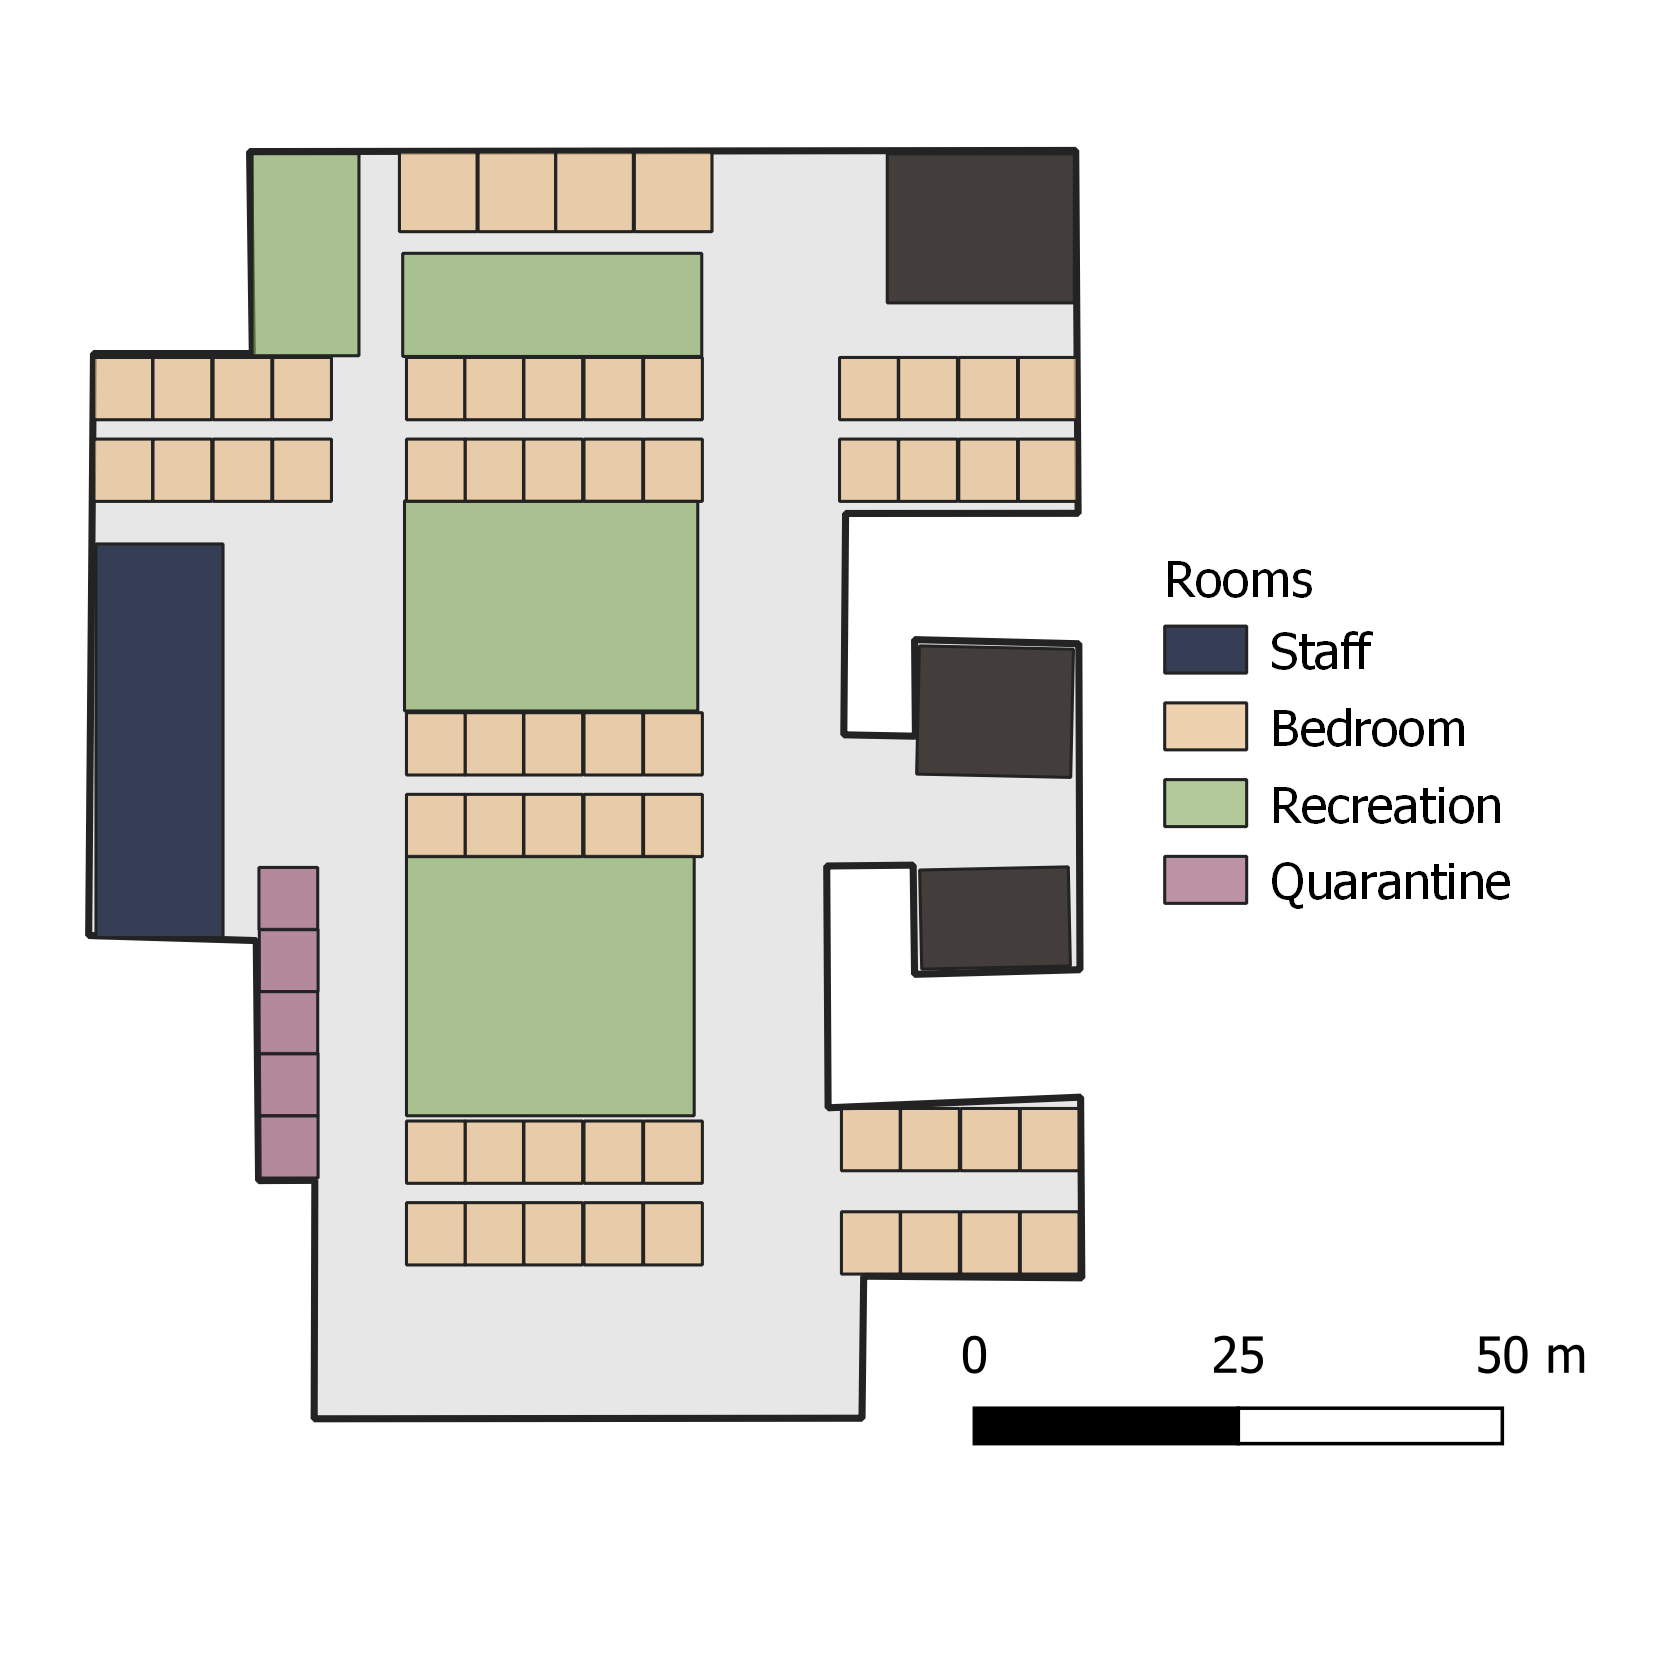
\includegraphics[width=8cm]{Figures/NH_B}
\end{figure}

\hypertarget{population-dynamics}{%
\subsubsection{Population dynamics}\label{population-dynamics}}

In our simulation, an agent can interact with other agents based on its
location. Given the current guidelines of recommendations for long term
care facilities, there are no visitations and the residents spend most
of the day in their rooms, so the resident agents in our simulation can
only interact with their roommates and the staff. The staff agents can
be one of three different types: Certified nurse (CN), Registered Nurses
(RN) or Licensed practical nurse (LPN). Our model allows to specify the
proportion of each type and work schedule for the staff agents.
Depending on the type, the staff agents will have different number of
contacts with the residents. The contact rates for each staff type were
parametrized based on the average number of resident contacts in a
regular day (REFERENCE: Table shared via email??). The staff agents are
assigned to one of 3 different work schedules (morning, afternoon or
night) and they spend 8 hours inside the nursery home and the rest of
the time outside in the community. We only follow the agents inside the
nursery home and when the agents are outside we assume that they all
have the same probability of contacting other people. The contact rates
and the staff schedule distribution used in our model are presented in
table from supplementary materials.

\begin{longtable}[]{@{}ll@{}}
\caption{Distribution of the Staff agent characteristics}\tabularnewline
\toprule
\begin{minipage}[b]{0.21\columnwidth}\raggedright
Variable\strut
\end{minipage} & \begin{minipage}[b]{0.73\columnwidth}\raggedright
Distribution\strut
\end{minipage}\tabularnewline
\midrule
\endfirsthead
\toprule
\begin{minipage}[b]{0.21\columnwidth}\raggedright
Variable\strut
\end{minipage} & \begin{minipage}[b]{0.73\columnwidth}\raggedright
Distribution\strut
\end{minipage}\tabularnewline
\midrule
\endhead
\begin{minipage}[t]{0.21\columnwidth}\raggedright
Work Schedule\strut
\end{minipage} & \begin{minipage}[t]{0.73\columnwidth}\raggedright
\(Multinom \sim (X_{morning} = 0.4, X_{Afternoon} = 0.4, X_{Night} = 0.2)\)\strut
\end{minipage}\tabularnewline
\begin{minipage}[t]{0.21\columnwidth}\raggedright
Staff type\strut
\end{minipage} & \begin{minipage}[t]{0.73\columnwidth}\raggedright
\(Multinom \sim (X_{CN} = 0.6, X_{RN} = 0.15, X_{LPN} = 0.15)\)\strut
\end{minipage}\tabularnewline
\begin{minipage}[t]{0.21\columnwidth}\raggedright
CN contacts per hour\strut
\end{minipage} & \begin{minipage}[t]{0.73\columnwidth}\raggedright
\(Multinom \sim (X_0 = 0.7, X_1 = 0.3)\)\strut
\end{minipage}\tabularnewline
\begin{minipage}[t]{0.21\columnwidth}\raggedright
RN contacts per hour\strut
\end{minipage} & \begin{minipage}[t]{0.73\columnwidth}\raggedright
\(Multinom \sim (X_0 = 0.25, X_1 = 0.75)\)\strut
\end{minipage}\tabularnewline
\begin{minipage}[t]{0.21\columnwidth}\raggedright
LPN contacts per hour\strut
\end{minipage} & \begin{minipage}[t]{0.73\columnwidth}\raggedright
\(Multinom \sim (X_0 = 0.15, X_2 = 0.2, X_3 = 0.25, X_4 = 0.2, X_5 = 0.2)\)\strut
\end{minipage}\tabularnewline
\bottomrule
\end{longtable}

\hypertarget{disease-dynamics}{%
\subsubsection{Disease dynamics:}\label{disease-dynamics}}

The transmission between agents inside the facility will depend on two
parts, which are the probability that a person will shed the virus and
the probability that another person will get the virus.This transmission
rates represent the probability that given that two individuals are in
the same room for 1 hour are going to shed or infect with the virus
depending on their disease state. We decided on model the transmission
this way to represent scenarios where the infected and susceptible could
have different combination of interventions (i.e.~only infected received
the intervention, only susceptible received the intervention, both
received the intervention, etc..). The parametrization of the
transmission parameters was based on observed outbreaks in nursery homes
in California.

The introduction from the community to the facility depends on a
parameter \emph{Introduction\_p} that represents the chance that one of
the staff members will get infected from the disease at the community.

All the agents start as susceptible and after 1 day there is a resident
introduced with the disease. Then we follow up for 150 days or until the
disease has been absent for more than 14 simulation days. Once the
transmission between a infectious agent to a susceptible agent has been
successful, the susceptible agent becomes exposed and based on a
distribution for the latent period \(\lambda\), the agent becomes
infectious after \(\lambda\) number of days, which can be either
symptomatic and asymptomatic. The agent can infect other agents only
when its in the Infectious state, then they remain infectious during 15
days and they transition to recovered. The agents can transition to
infectious to hospitalized at any moment based on the hospitalization
rate. When the agents has been recovered they acquire infection
immunity, which lasts for 120 days.

\begin{figure}
\caption{Disease states}
\centering
\includegraphics[width=10cm]{Figures/DiseaseDynamics}
\end{figure}

\begin{longtable}[]{@{}lll@{}}
\caption{Disease parameters. \(^a\)Explored for sensitivity analysis and
scenario modeling, \(^b\)truncated distribution between a boundary of
reasonable values, \(^c\)fitted to a distribution}\tabularnewline
\toprule
Name & Value & Reference\tabularnewline
\midrule
\endfirsthead
\toprule
Name & Value & Reference\tabularnewline
\midrule
\endhead
Latent period (\(\lambda\)) & \(Lognormal(7, 3)\) & (He et al.
2020)\(^{b,c}\)\tabularnewline
Shedding probability & \(0.45\) & \(^a\)\tabularnewline
Infection probability & \(0.45\) & \(^a\)\tabularnewline
Introduction probability & \(0.5\) & \(^a\)\tabularnewline
Asymptomatic probability & \(0.25\) & \(^a\)\tabularnewline
Infection duration & \(15\ days\) &\tabularnewline
Hospitalization rate & \(0.11\) &\tabularnewline
\bottomrule
\end{longtable}

\hypertarget{interventions}{%
\subsection{Interventions}\label{interventions}}

We explore 3 different COVID-19 control strategies and the combination
of them. Each of the interventions have an impact in the transmission of
the disease, interventions such as the use of PPE and vaccination
reduces the probability of transmission affecting directly the
\emph{Shedding} and \emph{Infection probability}, while the isolation
affects the transmission indirectly stopping the agent to interact with
other agents. The equation 1 shows the effect of \emph{PPE effect} and
\emph{Vaccine effect} on the transmission probability, where
\(odds_\omega\) represent the global transmission probability for all
agents, \(OR_\pi\) represent the odds ratio for the \emph{PPE effect},
\(X_\pi\) represent the presence or absence of PPE, \(OR\upsilon\) is
the \emph{Vaccine effect}, and \(X_\upsilon\). This probability is
computed for all agents at each step so we can have different
probabilities of transmission based on the interventions each individual
received.

\[p_T = \frac{e^{\ln(odds_\omega) + \ln(OR_\pi X_\pi)+ \ln(OR_\upsilon X_\upsilon)}}{1 + e^{\ln(odds_\omega) + \ln(OR_\pi X_\pi)+ \ln(OR_\upsilon  X_\upsilon)}}\]
For the implementation of the vaccination, we specified by the
proportion of residents and staff vaccinated, and a fixed interval
between the first and second dose of 21 days. After the first dose, the
agents will only obtain a 60\% of the total immunity protection assumed
to be conferred by the vaccine, then on the second dose the agents will
have 100\% of the assumed effect. Then the vaccination immunity will
have a decay of 120 days and the individual will no longer have the
vaccination immunity protective effect.

Since there is still some uncertainty in the effect of the use of PPE
and the vaccine for older population, we started with values that are
within the range of reported values and then varied these values for the
sensitivity analysis and scenario modeling.

\hypertarget{testing-and-isolation}{%
\subsubsection{Testing and isolation}\label{testing-and-isolation}}

Other models have explored this more in detail, in our model we wanted
to simplify and used this detection probability parameter to represent
the chance that an individual that is tested for the disease will be
correctly identified regardless which test is used.\\
Our model represents the testing of the population with 2 different
approaches:

\begin{itemize}
\tightlist
\item
  Reactive, individuals are tested once that they present symptoms, this
  approach is focused on the early detection of symptomatic individuals.
\item
  Proactive, a proportion of individuals are tested with a given
  frequency. In baseline scenario, 1 resident per room and all the staff
  are tested weekly. If 1 of the residents in a room is detected
  positive, the rest of the residents in that room are also tested.
\end{itemize}

Once a individual has been detected positive is isolated. There are
special isolation rooms for the residents and in the case of the staff
they are sent home. Once the individual is tested negative they return
to the facility.

Interventions parameters:

\begin{longtable}[]{@{}lll@{}}
\caption{Interventions parameters. \(^a\)Explored for sensitivity
analysis and scenario modeling, \(^b\)truncated distribution between a
boundary of reasonable values, \(^c\)fitted to a
distribution}\tabularnewline
\toprule
Name & Value & Reference\tabularnewline
\midrule
\endfirsthead
\toprule
Name & Value & Reference\tabularnewline
\midrule
\endhead
Proportion of staff using PPE & 0.9 & \(^a\)\tabularnewline
Proportion of residents using PPE & 0.75 & \(^a\)\tabularnewline
PPE Effect (\(OR_\pi\)) & 0.34089 & (Chu et al.
2020)\(^a\)\tabularnewline
Test detection probability & \(80\%\) & \(^a\)\tabularnewline
Proportion of Staff tested & \(90\%\) & \(^a\)\tabularnewline
Proportion of Residents tested & \(33.3%
\) & \(^a\)\tabularnewline
Frequency of testing & Weekly & \(^a\)\tabularnewline
Vaccine effect (\(OR_\upsilon\)) & 0.0493 & (Pfizer-BioNTech
2020)\(^a\)\tabularnewline
Vaccine immunity duration & \(120\ days\) & \(^a\)\tabularnewline
\bottomrule
\end{longtable}

\hypertarget{sensitivity-analysis}{%
\subsection{Sensitivity analysis}\label{sensitivity-analysis}}

We performed sensitivity analysis on selected parameters to show the
influence of these parameters on the outcomes. We present the disease
outcomes from our model summarized using plots and median and 95\%
confidence intervals for the days until the facility became disease
free, infection rate, cumulative number of infected staff and residents
and cumulative number of hospitalizations.

\begin{longtable}[]{@{}lll@{}}
\caption{Parameters used for sensitivity analysis}\tabularnewline
\toprule
Scenario & Target parameter & Value used\tabularnewline
\midrule
\endfirsthead
\toprule
Scenario & Target parameter & Value used\tabularnewline
\midrule
\endhead
Low transmission & Shedding and infection probability &
0.4\tabularnewline
High transmission & Shedding and infection probability &
0.4\tabularnewline
Low Introduction Probability & Introduction probability &
0.01\tabularnewline
High Introduction Probability & Introduction probability &
0.15\tabularnewline
Low Detection Probability & Detection probability & 0.75\tabularnewline
High Detection Probability & Detection probability & 0.90\tabularnewline
High effect PPE & PPE effect & 0.0493\tabularnewline
Low effect PPE & PPE effect & 0.3408\tabularnewline
Every 5 days & Testing frequency & every 5 days\tabularnewline
Every 3 days & Testing frequency & every 3 days\tabularnewline
\bottomrule
\end{longtable}

\hypertarget{effect-of-vaccination}{%
\subsubsection{Effect of vaccination}\label{effect-of-vaccination}}

To effect of the vaccine on reducing the transmission we parametrized
the model according to the current vaccine effect reported by the trials
from the Moderna and Pfizer vaccine (Baden et al. 2020; Polack et al.
2020). Since there is still some uncertainty about the effect of the
vaccine in population \textgreater65 years, we defined 3 scenarios that
explore the possible outcomes under 3 different assumptions:

\begin{itemize}
\tightlist
\item
  Equal effect: The vaccine has the same effect both populations
  (\textgreater65 years and \textgreater65 years).
\item
  Pfizer: The vaccine is less effective on populations \textgreater65
  years parametrized according to the reported by (Baden et al. 2020).
\item
  Moderna: The vaccine is less effective on populations \textgreater65
  years parametrized according to the reported by (Polack et al. 2020).
\end{itemize}

\begin{longtable}[]{@{}llll@{}}
\caption{Vaccine effect scenarios}\tabularnewline
\toprule
Scenario & \(OR_{V,S}\) & \(OR_{V,R}\) & Reference\tabularnewline
\midrule
\endfirsthead
\toprule
Scenario & \(OR_{V,S}\) & \(OR_{V,R}\) & Reference\tabularnewline
\midrule
\endhead
Equal effect & 0.0493 & 0.0493 & (Baden et al. 2020)\tabularnewline
Pfizer & 0.0434 & 0.0619 & (Baden et al. 2020)\tabularnewline
Moderna & 0.0441 & 0.1357 & (Polack et al. 2020)\tabularnewline
\bottomrule
\end{longtable}

\hypertarget{vaccine-distribution}{%
\subsubsection{Vaccine distribution}\label{vaccine-distribution}}

\hypertarget{scenario-modeling}{%
\subsubsection{Scenario modeling}\label{scenario-modeling}}

To illustrate the applications of our model we wanted to answer the
question ``How should the resources should be distributed under two
different levels of community transmission?''. We defined as a low
community transmission where the probability of introduction is 1\% and
high community transmission where the probability of introduction is
5\%. Then we used the worst case scenario for the effect of the vaccine
on the two age groups and looked at the disease outcomes including
infection rate and time to duration of the outbreak.

\hypertarget{results}{%
\section{Results}\label{results}}

\hypertarget{baseline-scenario}{%
\subsection{Baseline scenario}\label{baseline-scenario}}

The baseline scenario follows the current interventions implemented in a
typical nursery home. The parameters for the population dynamics,
disease transmission and interventions effect used for the baseline
scenario are the ones presented on the tables 1, 2, and 3 respectively.
Testing is performed once a week to all the staff and one resident per
room. Once that the resident is detected positive is sent to a isolation
room, and in the case that one of the staff members test positive, it
will be send home. Both the staff and residents are required to use PPE.

The baseline scenarios is meant to represent the possible outcomes for
an average nursery home under the current conditions in the US. Our
baseline scenario shows a wide range of disease impact ranging from 7-56
days to disease control, and an infection rate ranging between 0.01 to
0.56.

\begin{figure}
\caption{Baseline scenario}
\centering
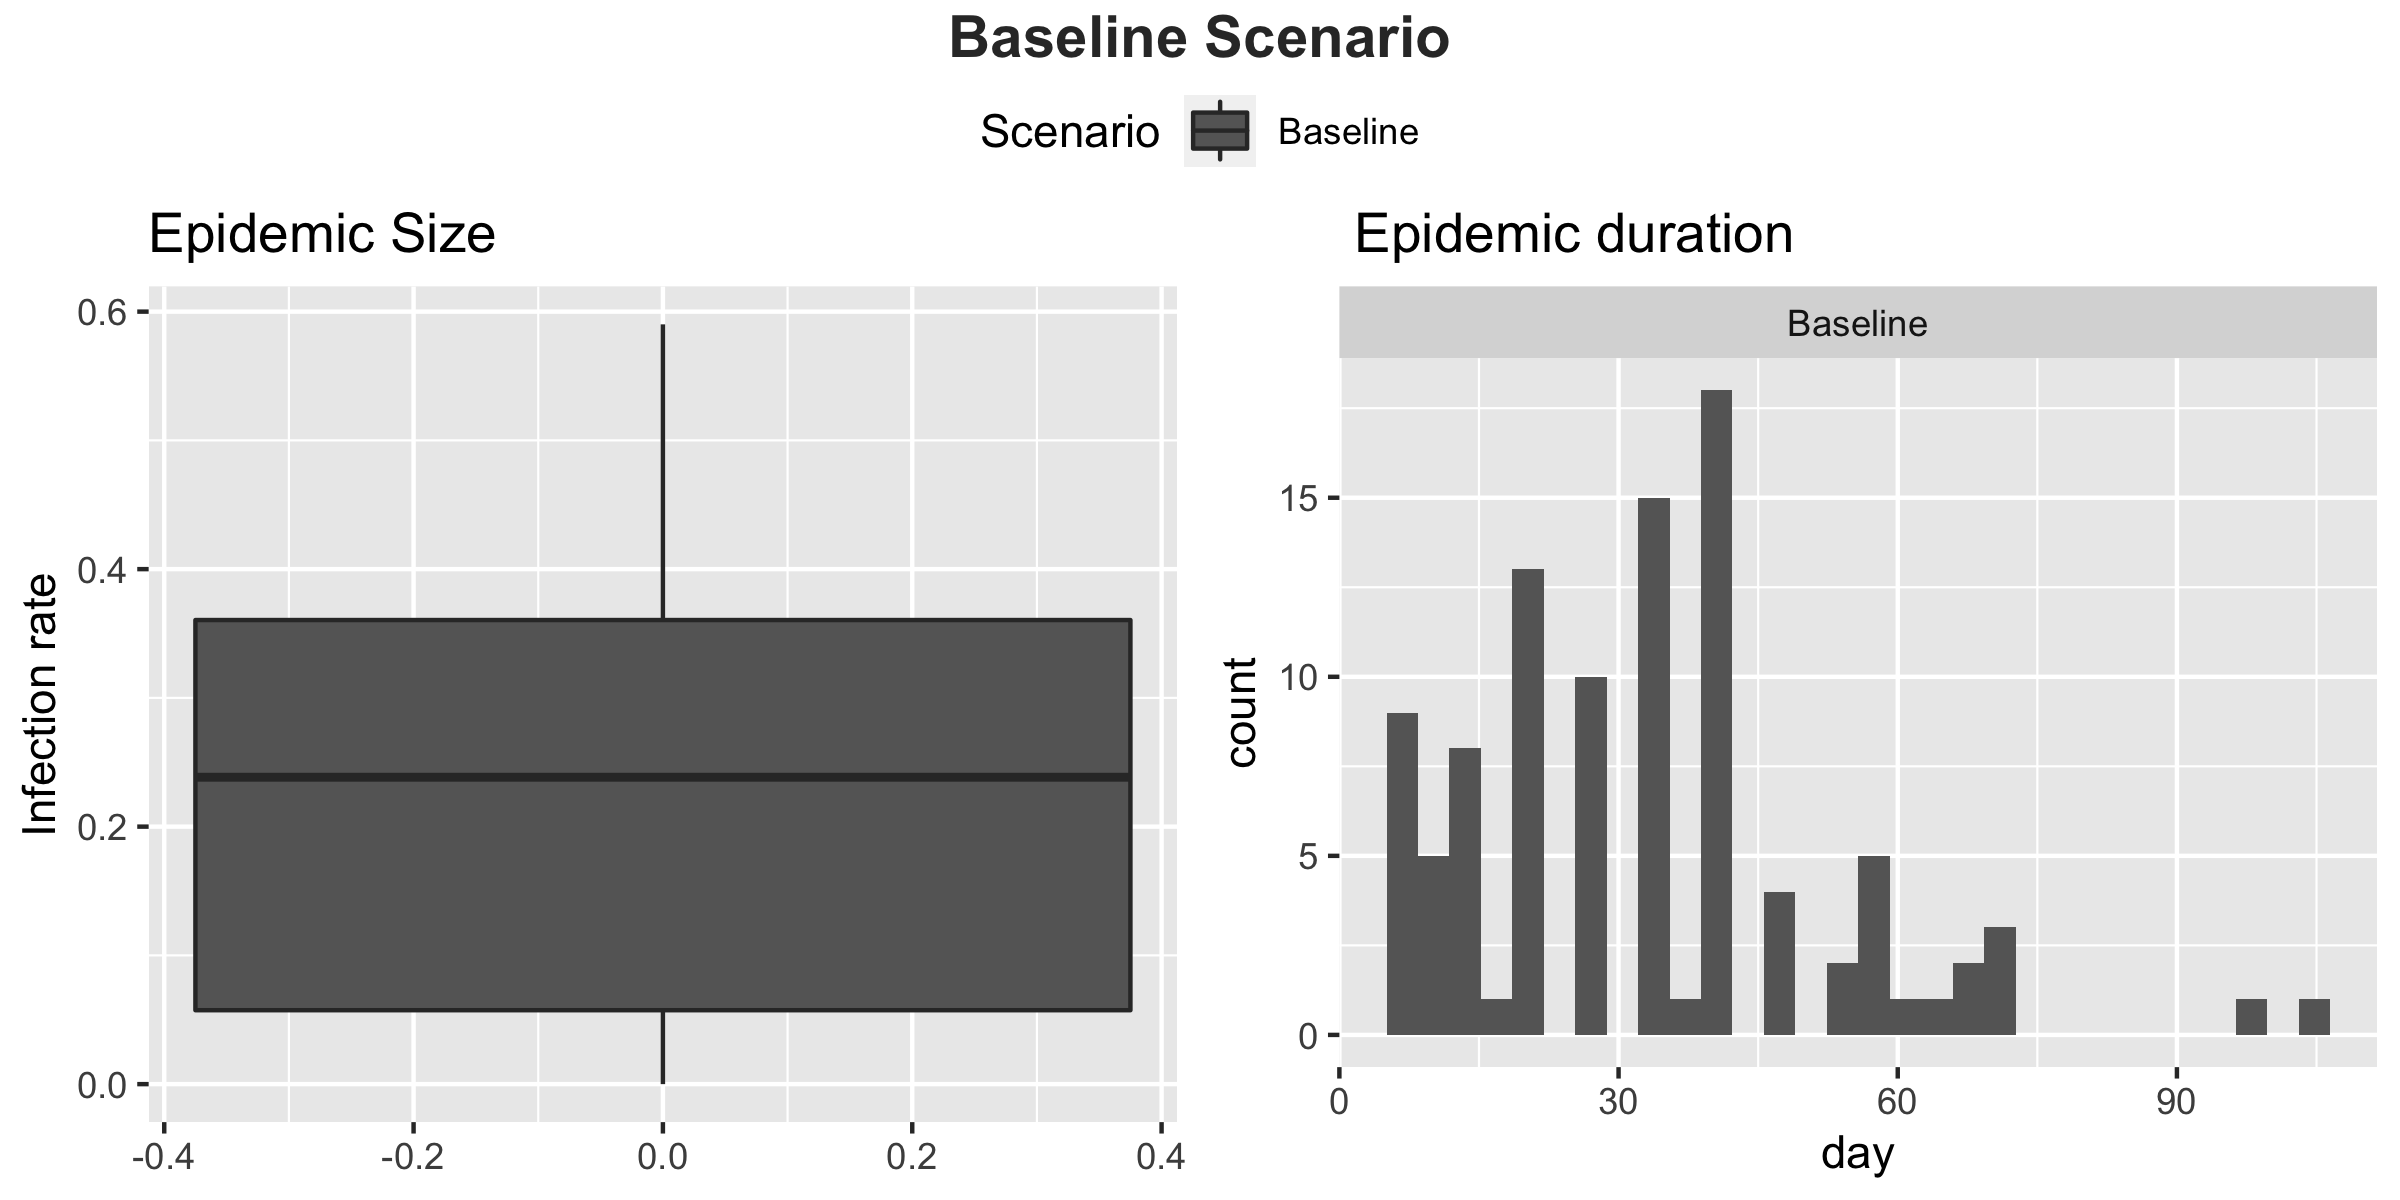
\includegraphics{Figures/SensitivityAnalysis/Baseline}
\end{figure}

\hypertarget{sensitivty-analisis}{%
\subsection{Sensitivty analisis}\label{sensitivty-analisis}}

The influence of different parameters in our model outcomes are
presented in the table 6.

\begin{longtable}[]{@{}lllllll@{}}
\caption{Results from the sensitivity analysis using the median and 95\%
confidence intervals}\tabularnewline
\toprule
\begin{minipage}[b]{0.18\columnwidth}\raggedright
Scenario\strut
\end{minipage} & \begin{minipage}[b]{0.12\columnwidth}\raggedright
Days to eradication\strut
\end{minipage} & \begin{minipage}[b]{0.10\columnwidth}\raggedright
Infection rate\strut
\end{minipage} & \begin{minipage}[b]{0.11\columnwidth}\raggedright
Total Infected\strut
\end{minipage} & \begin{minipage}[b]{0.11\columnwidth}\raggedright
Infected residents\strut
\end{minipage} & \begin{minipage}[b]{0.09\columnwidth}\raggedright
Infected staff\strut
\end{minipage} & \begin{minipage}[b]{0.10\columnwidth}\raggedright
Hospitalizations\strut
\end{minipage}\tabularnewline
\midrule
\endfirsthead
\toprule
\begin{minipage}[b]{0.18\columnwidth}\raggedright
Scenario\strut
\end{minipage} & \begin{minipage}[b]{0.12\columnwidth}\raggedright
Days to eradication\strut
\end{minipage} & \begin{minipage}[b]{0.10\columnwidth}\raggedright
Infection rate\strut
\end{minipage} & \begin{minipage}[b]{0.11\columnwidth}\raggedright
Total Infected\strut
\end{minipage} & \begin{minipage}[b]{0.11\columnwidth}\raggedright
Infected residents\strut
\end{minipage} & \begin{minipage}[b]{0.09\columnwidth}\raggedright
Infected staff\strut
\end{minipage} & \begin{minipage}[b]{0.10\columnwidth}\raggedright
Hospitalizations\strut
\end{minipage}\tabularnewline
\midrule
\endhead
\begin{minipage}[t]{0.18\columnwidth}\raggedright
Baseline\strut
\end{minipage} & \begin{minipage}[t]{0.12\columnwidth}\raggedright
28 (7,56)\strut
\end{minipage} & \begin{minipage}[t]{0.10\columnwidth}\raggedright
0.34 (0.01,0.56)\strut
\end{minipage} & \begin{minipage}[t]{0.11\columnwidth}\raggedright
117 (3,192.6)\strut
\end{minipage} & \begin{minipage}[t]{0.11\columnwidth}\raggedright
72 (0.4,125.2)\strut
\end{minipage} & \begin{minipage}[t]{0.09\columnwidth}\raggedright
44 (2.6,76.6)\strut
\end{minipage} & \begin{minipage}[t]{0.10\columnwidth}\raggedright
29 (0.2,55.4)\strut
\end{minipage}\tabularnewline
\begin{minipage}[t]{0.18\columnwidth}\raggedright
Low transmission\strut
\end{minipage} & \begin{minipage}[t]{0.12\columnwidth}\raggedright
28 (7,59.2)\strut
\end{minipage} & \begin{minipage}[t]{0.10\columnwidth}\raggedright
0.17 (0.01,0.38)\strut
\end{minipage} & \begin{minipage}[t]{0.11\columnwidth}\raggedright
58 (2.2,130.8)\strut
\end{minipage} & \begin{minipage}[t]{0.11\columnwidth}\raggedright
30 (0,88.4)\strut
\end{minipage} & \begin{minipage}[t]{0.09\columnwidth}\raggedright
26 (2,55.2)\strut
\end{minipage} & \begin{minipage}[t]{0.10\columnwidth}\raggedright
11 (1,34)\strut
\end{minipage}\tabularnewline
\begin{minipage}[t]{0.18\columnwidth}\raggedright
High transmission\strut
\end{minipage} & \begin{minipage}[t]{0.12\columnwidth}\raggedright
21 (10,42)\strut
\end{minipage} & \begin{minipage}[t]{0.10\columnwidth}\raggedright
0.5 (0.08,0.65)\strut
\end{minipage} & \begin{minipage}[t]{0.11\columnwidth}\raggedright
172 (27.4,224.6)\strut
\end{minipage} & \begin{minipage}[t]{0.11\columnwidth}\raggedright
102 (16.2,137.8)\strut
\end{minipage} & \begin{minipage}[t]{0.09\columnwidth}\raggedright
66 (11.2,88.6)\strut
\end{minipage} & \begin{minipage}[t]{0.10\columnwidth}\raggedright
32 (3.4,62.8)\strut
\end{minipage}\tabularnewline
\begin{minipage}[t]{0.18\columnwidth}\raggedright
Low Introduction Probability\strut
\end{minipage} & \begin{minipage}[t]{0.12\columnwidth}\raggedright
16 (9,40.6)\strut
\end{minipage} & \begin{minipage}[t]{0.10\columnwidth}\raggedright
0.08 (0,0.48)\strut
\end{minipage} & \begin{minipage}[t]{0.11\columnwidth}\raggedright
27 (0,166.2)\strut
\end{minipage} & \begin{minipage}[t]{0.11\columnwidth}\raggedright
13 (0,109.4)\strut
\end{minipage} & \begin{minipage}[t]{0.09\columnwidth}\raggedright
14 (0,59.4)\strut
\end{minipage} & \begin{minipage}[t]{0.10\columnwidth}\raggedright
8 (0.2,44.2)\strut
\end{minipage}\tabularnewline
\begin{minipage}[t]{0.18\columnwidth}\raggedright
High Introduction Probability\strut
\end{minipage} & \begin{minipage}[t]{0.12\columnwidth}\raggedright
28 (14,49)\strut
\end{minipage} & \begin{minipage}[t]{0.10\columnwidth}\raggedright
0.35 (0.05,0.55)\strut
\end{minipage} & \begin{minipage}[t]{0.11\columnwidth}\raggedright
120 (18.8,188.4)\strut
\end{minipage} & \begin{minipage}[t]{0.11\columnwidth}\raggedright
71 (8.2,118.2)\strut
\end{minipage} & \begin{minipage}[t]{0.09\columnwidth}\raggedright
48 (10.6,73.6)\strut
\end{minipage} & \begin{minipage}[t]{0.10\columnwidth}\raggedright
24 (4,47.4)\strut
\end{minipage}\tabularnewline
\begin{minipage}[t]{0.18\columnwidth}\raggedright
Low Detection Probability\strut
\end{minipage} & \begin{minipage}[t]{0.12\columnwidth}\raggedright
28 (9.6,57.8)\strut
\end{minipage} & \begin{minipage}[t]{0.10\columnwidth}\raggedright
0.42 (0.04,0.58)\strut
\end{minipage} & \begin{minipage}[t]{0.11\columnwidth}\raggedright
145 (14.8,199.2)\strut
\end{minipage} & \begin{minipage}[t]{0.11\columnwidth}\raggedright
91 (7.6,124.4)\strut
\end{minipage} & \begin{minipage}[t]{0.09\columnwidth}\raggedright
56 (7.2,77.2)\strut
\end{minipage} & \begin{minipage}[t]{0.10\columnwidth}\raggedright
25 (3,48)\strut
\end{minipage}\tabularnewline
\begin{minipage}[t]{0.18\columnwidth}\raggedright
High Detection Probability\strut
\end{minipage} & \begin{minipage}[t]{0.12\columnwidth}\raggedright
21 (7,46.8)\strut
\end{minipage} & \begin{minipage}[t]{0.10\columnwidth}\raggedright
0.24 (0.01,0.44)\strut
\end{minipage} & \begin{minipage}[t]{0.11\columnwidth}\raggedright
81 (2.2,150.6)\strut
\end{minipage} & \begin{minipage}[t]{0.11\columnwidth}\raggedright
45 (0,92.2)\strut
\end{minipage} & \begin{minipage}[t]{0.09\columnwidth}\raggedright
26 (2.2,58.4)\strut
\end{minipage} & \begin{minipage}[t]{0.10\columnwidth}\raggedright
7 (0.2,29.4)\strut
\end{minipage}\tabularnewline
\begin{minipage}[t]{0.18\columnwidth}\raggedright
High effect PPE\strut
\end{minipage} & \begin{minipage}[t]{0.12\columnwidth}\raggedright
16 (7,53.2)\strut
\end{minipage} & \begin{minipage}[t]{0.10\columnwidth}\raggedright
0.03 (0,0.26)\strut
\end{minipage} & \begin{minipage}[t]{0.11\columnwidth}\raggedright
11 (1,88.2)\strut
\end{minipage} & \begin{minipage}[t]{0.11\columnwidth}\raggedright
2 (0,55.4)\strut
\end{minipage} & \begin{minipage}[t]{0.09\columnwidth}\raggedright
9 (1,35.4)\strut
\end{minipage} & \begin{minipage}[t]{0.10\columnwidth}\raggedright
1 (0,21.4)\strut
\end{minipage}\tabularnewline
\begin{minipage}[t]{0.18\columnwidth}\raggedright
Low effect PPE\strut
\end{minipage} & \begin{minipage}[t]{0.12\columnwidth}\raggedright
21 (14,28)\strut
\end{minipage} & \begin{minipage}[t]{0.10\columnwidth}\raggedright
0.83 (0.6,1.03)\strut
\end{minipage} & \begin{minipage}[t]{0.11\columnwidth}\raggedright
285 (207.4,354.6)\strut
\end{minipage} & \begin{minipage}[t]{0.11\columnwidth}\raggedright
177 (124.6,221.4)\strut
\end{minipage} & \begin{minipage}[t]{0.09\columnwidth}\raggedright
111 (87.6,140)\strut
\end{minipage} & \begin{minipage}[t]{0.10\columnwidth}\raggedright
48 (20.4,71.4)\strut
\end{minipage}\tabularnewline
\begin{minipage}[t]{0.18\columnwidth}\raggedright
Every 5 days\strut
\end{minipage} & \begin{minipage}[t]{0.12\columnwidth}\raggedright
20 (5,78.2)\strut
\end{minipage} & \begin{minipage}[t]{0.10\columnwidth}\raggedright
0.19 (0.01,0.42)\strut
\end{minipage} & \begin{minipage}[t]{0.11\columnwidth}\raggedright
65 (2,144)\strut
\end{minipage} & \begin{minipage}[t]{0.11\columnwidth}\raggedright
39 (0,87.2)\strut
\end{minipage} & \begin{minipage}[t]{0.09\columnwidth}\raggedright
29 (1.2,59.2)\strut
\end{minipage} & \begin{minipage}[t]{0.10\columnwidth}\raggedright
14 (0.2,31.8)\strut
\end{minipage}\tabularnewline
\begin{minipage}[t]{0.18\columnwidth}\raggedright
Every 3 days\strut
\end{minipage} & \begin{minipage}[t]{0.12\columnwidth}\raggedright
0 (0,6)\strut
\end{minipage} & \begin{minipage}[t]{0.10\columnwidth}\raggedright
0 (0,0.01)\strut
\end{minipage} & \begin{minipage}[t]{0.11\columnwidth}\raggedright
0 (0,2)\strut
\end{minipage} & \begin{minipage}[t]{0.11\columnwidth}\raggedright
0 (0,0)\strut
\end{minipage} & \begin{minipage}[t]{0.09\columnwidth}\raggedright
0 (0,1)\strut
\end{minipage} & \begin{minipage}[t]{0.10\columnwidth}\raggedright
0 (0,0)\strut
\end{minipage}\tabularnewline
\begin{minipage}[t]{0.18\columnwidth}\raggedright
Same vaccine effect\strut
\end{minipage} & \begin{minipage}[t]{0.12\columnwidth}\raggedright
14 (7,35)\strut
\end{minipage} & \begin{minipage}[t]{0.10\columnwidth}\raggedright
0.02 (0,0.13)\strut
\end{minipage} & \begin{minipage}[t]{0.11\columnwidth}\raggedright
6 (0.2,46)\strut
\end{minipage} & \begin{minipage}[t]{0.11\columnwidth}\raggedright
1 (0,25.4)\strut
\end{minipage} & \begin{minipage}[t]{0.09\columnwidth}\raggedright
5 (0.2,21.8)\strut
\end{minipage} & \begin{minipage}[t]{0.10\columnwidth}\raggedright
1 (0,7.4)\strut
\end{minipage}\tabularnewline
\begin{minipage}[t]{0.18\columnwidth}\raggedright
Pfizer\strut
\end{minipage} & \begin{minipage}[t]{0.12\columnwidth}\raggedright
14 (7,32)\strut
\end{minipage} & \begin{minipage}[t]{0.10\columnwidth}\raggedright
0.02 (0,0.12)\strut
\end{minipage} & \begin{minipage}[t]{0.11\columnwidth}\raggedright
6 (0.2,41.8)\strut
\end{minipage} & \begin{minipage}[t]{0.11\columnwidth}\raggedright
1 (0,24.6)\strut
\end{minipage} & \begin{minipage}[t]{0.09\columnwidth}\raggedright
5 (0.2,17.2)\strut
\end{minipage} & \begin{minipage}[t]{0.10\columnwidth}\raggedright
1 (0,9.6)\strut
\end{minipage}\tabularnewline
\begin{minipage}[t]{0.18\columnwidth}\raggedright
Moderna\strut
\end{minipage} & \begin{minipage}[t]{0.12\columnwidth}\raggedright
14 (7,33.6)\strut
\end{minipage} & \begin{minipage}[t]{0.10\columnwidth}\raggedright
0.02 (0,0.15)\strut
\end{minipage} & \begin{minipage}[t]{0.11\columnwidth}\raggedright
6 (0,50.6)\strut
\end{minipage} & \begin{minipage}[t]{0.11\columnwidth}\raggedright
1 (0,26)\strut
\end{minipage} & \begin{minipage}[t]{0.09\columnwidth}\raggedright
5 (0,22.2)\strut
\end{minipage} & \begin{minipage}[t]{0.10\columnwidth}\raggedright
1 (0,6.8)\strut
\end{minipage}\tabularnewline
\begin{minipage}[t]{0.18\columnwidth}\raggedright
Resident priority\strut
\end{minipage} & \begin{minipage}[t]{0.12\columnwidth}\raggedright
9 (7,26.6)\strut
\end{minipage} & \begin{minipage}[t]{0.10\columnwidth}\raggedright
0.01 (0,0.08)\strut
\end{minipage} & \begin{minipage}[t]{0.11\columnwidth}\raggedright
4 (0,27)\strut
\end{minipage} & \begin{minipage}[t]{0.11\columnwidth}\raggedright
1 (0,13.6)\strut
\end{minipage} & \begin{minipage}[t]{0.09\columnwidth}\raggedright
3 (0,15.6)\strut
\end{minipage} & \begin{minipage}[t]{0.10\columnwidth}\raggedright
1 (0,6.2)\strut
\end{minipage}\tabularnewline
\begin{minipage}[t]{0.18\columnwidth}\raggedright
Staff priority\strut
\end{minipage} & \begin{minipage}[t]{0.12\columnwidth}\raggedright
21 (7,34.8)\strut
\end{minipage} & \begin{minipage}[t]{0.10\columnwidth}\raggedright
0.03 (0,0.18)\strut
\end{minipage} & \begin{minipage}[t]{0.11\columnwidth}\raggedright
9 (1.2,60.4)\strut
\end{minipage} & \begin{minipage}[t]{0.11\columnwidth}\raggedright
3 (0,44.2)\strut
\end{minipage} & \begin{minipage}[t]{0.09\columnwidth}\raggedright
5 (1.2,21.4)\strut
\end{minipage} & \begin{minipage}[t]{0.10\columnwidth}\raggedright
1 (0,9.6)\strut
\end{minipage}\tabularnewline
\bottomrule
\end{longtable}

\begin{figure}
\caption{Sensitivity analysis on the transmission parameter}
\centering
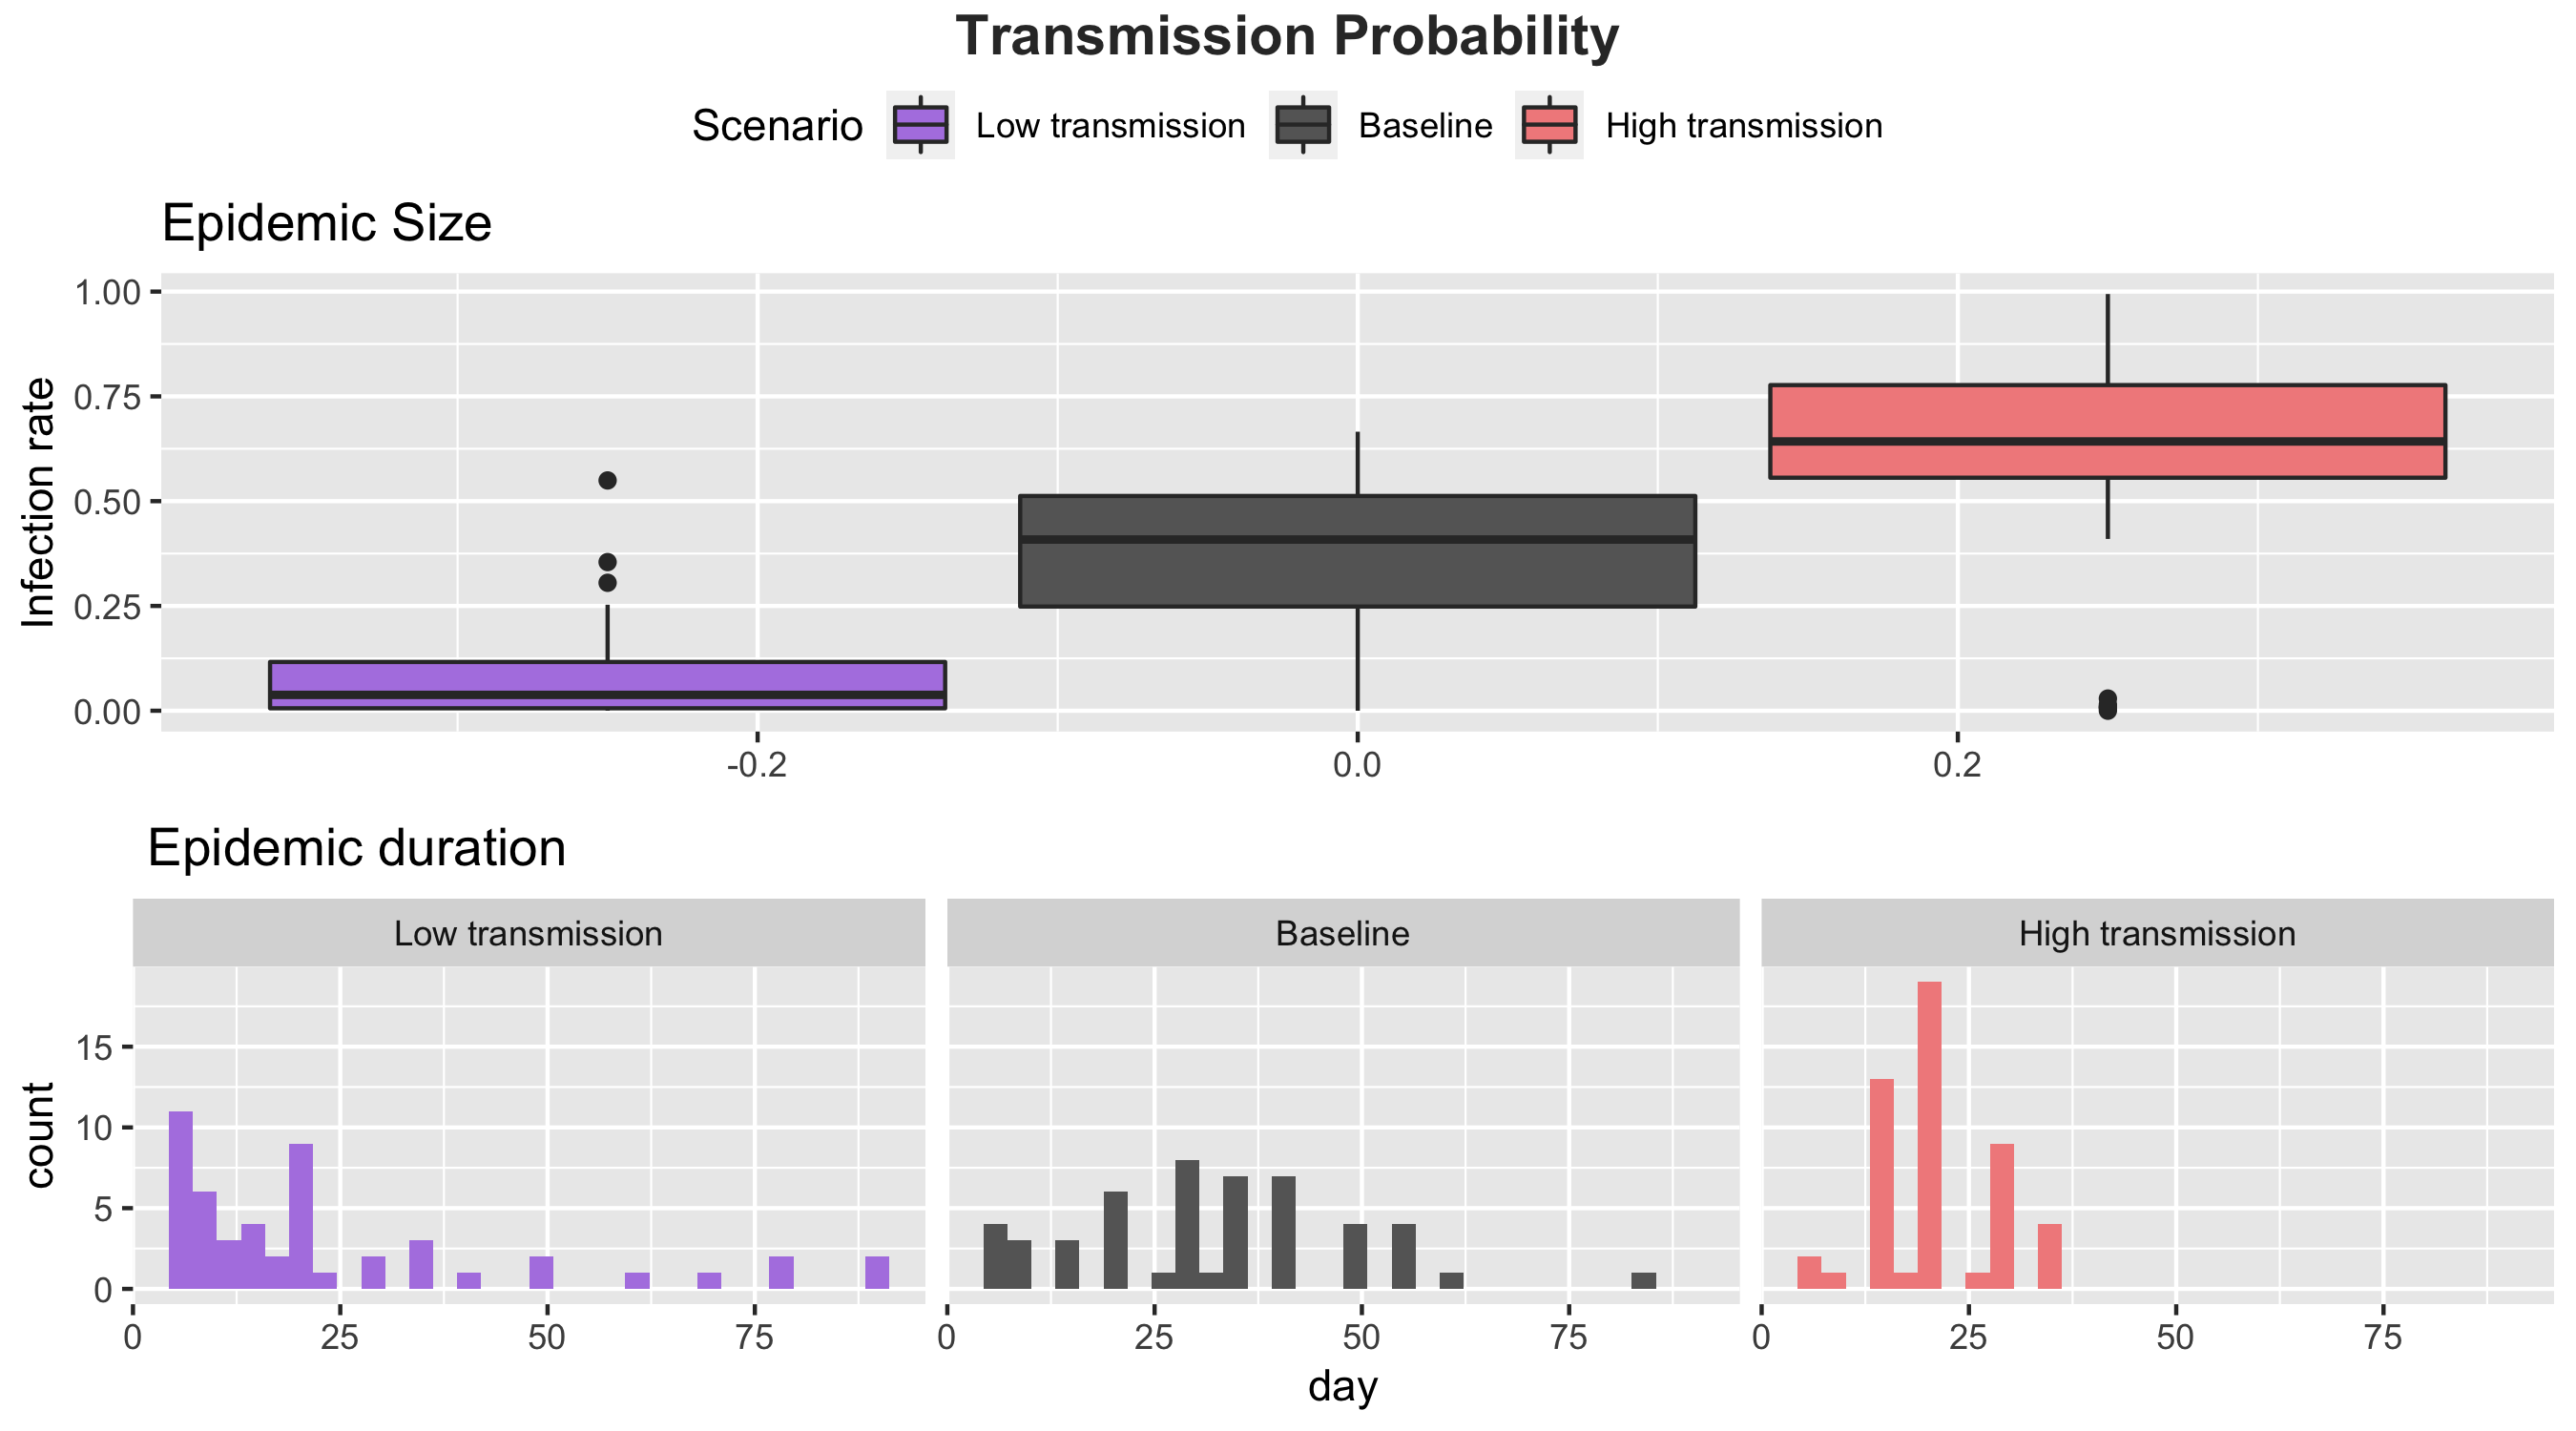
\includegraphics{Figures/SensitivityAnalysis/Transmission}  
\end{figure}

\begin{figure}
\caption{Sensitivity analysis on the introduction probability}
\centering
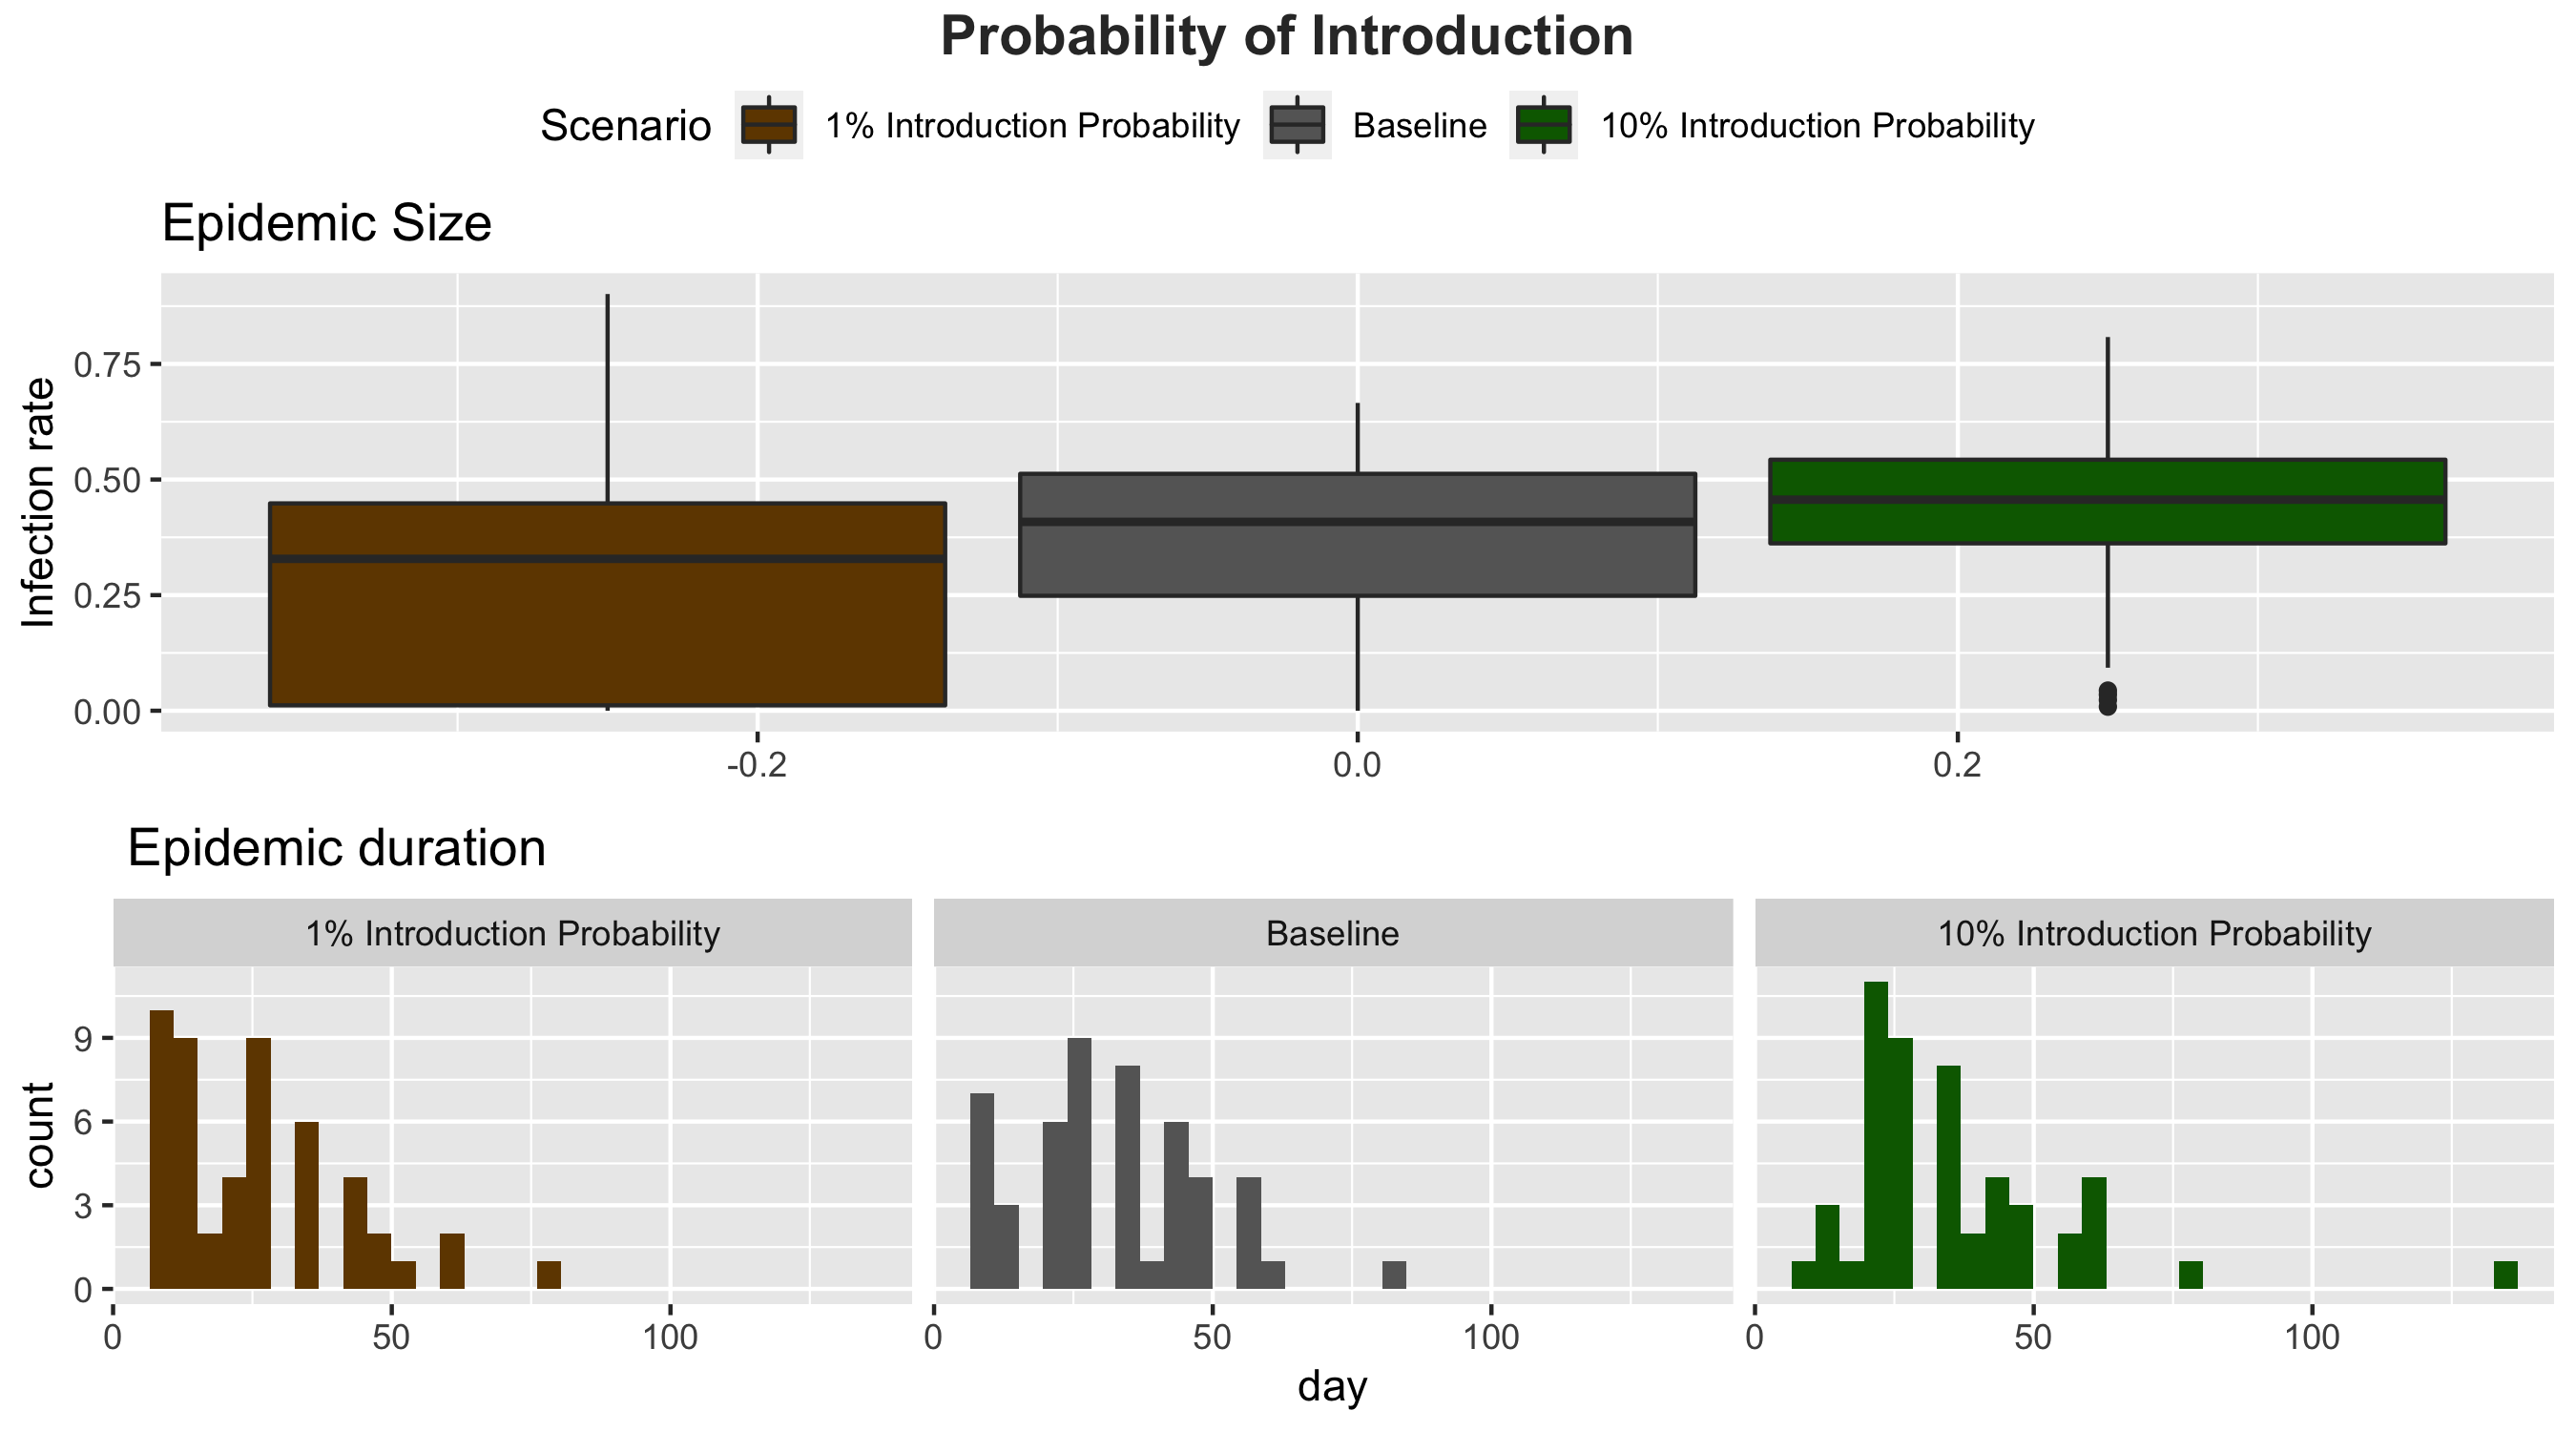
\includegraphics{Figures/SensitivityAnalysis/Introduction}  
\end{figure}

\begin{figure}
\caption{Sensitivity analysis on the probability of detection}
\centering
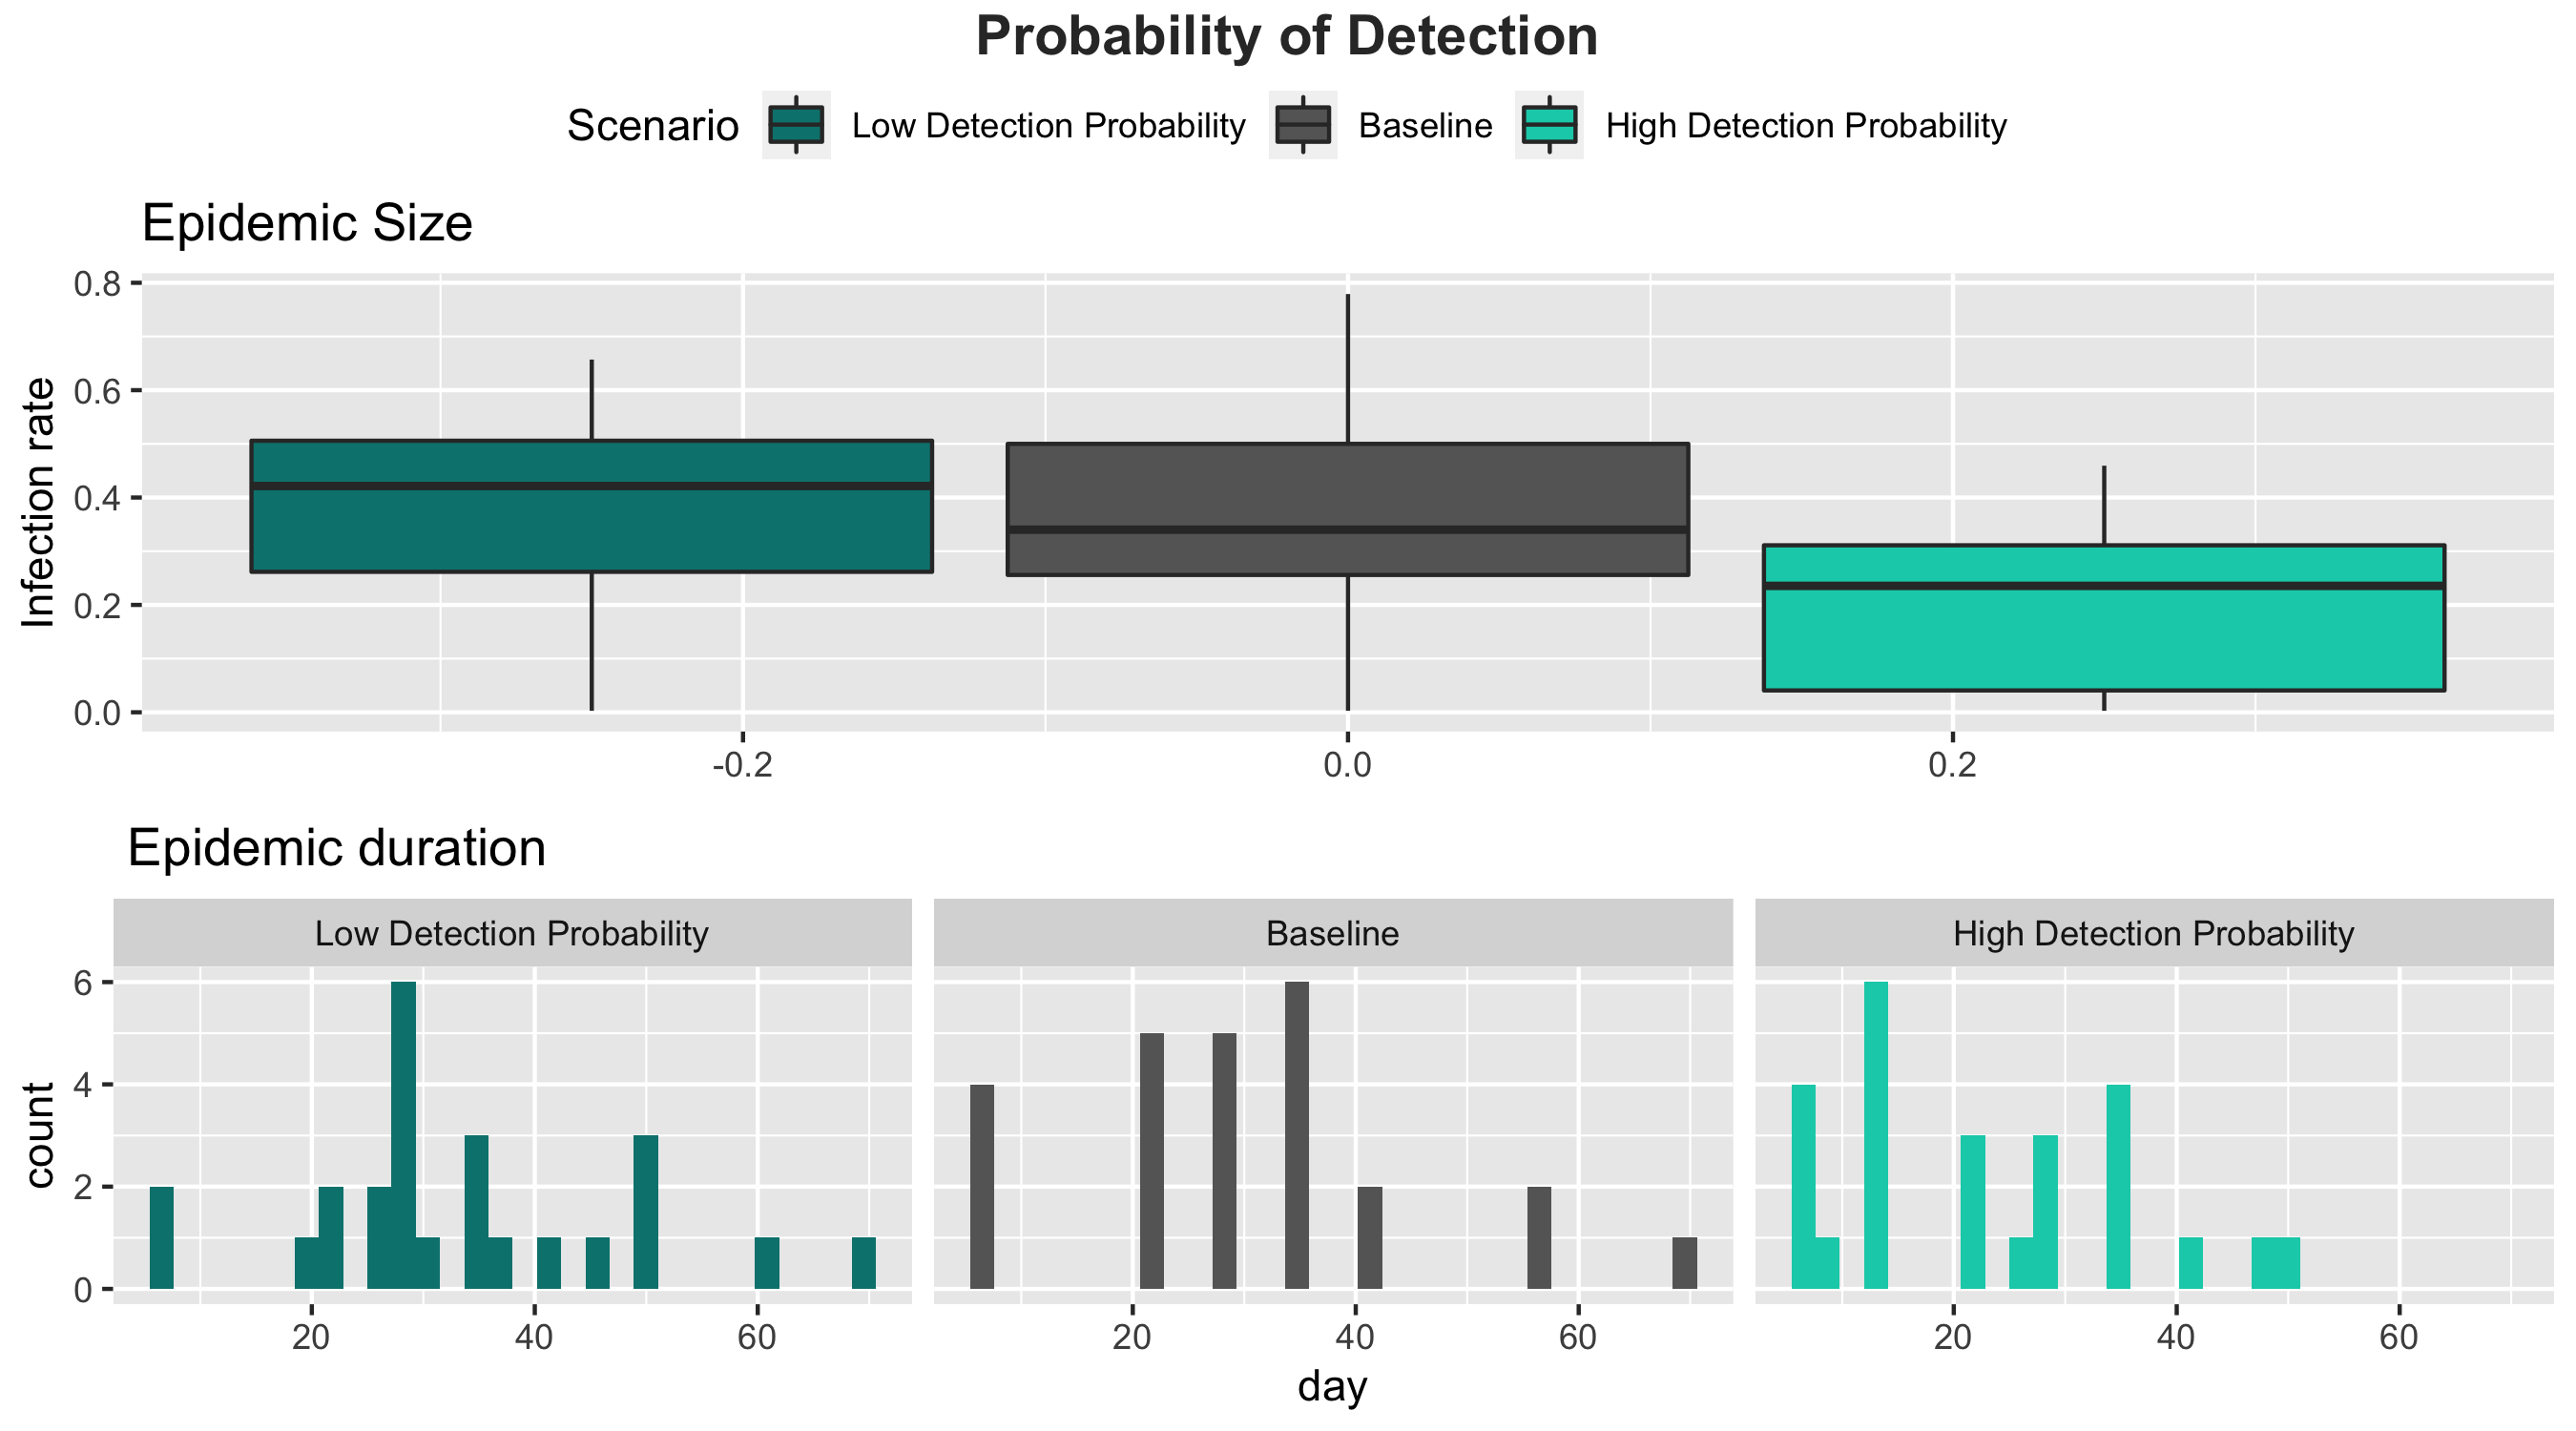
\includegraphics{Figures/SensitivityAnalysis/ProbDetection}  
\end{figure}

\begin{figure}
\caption{Sensitivity analysis on the effect of the PPE}
\centering
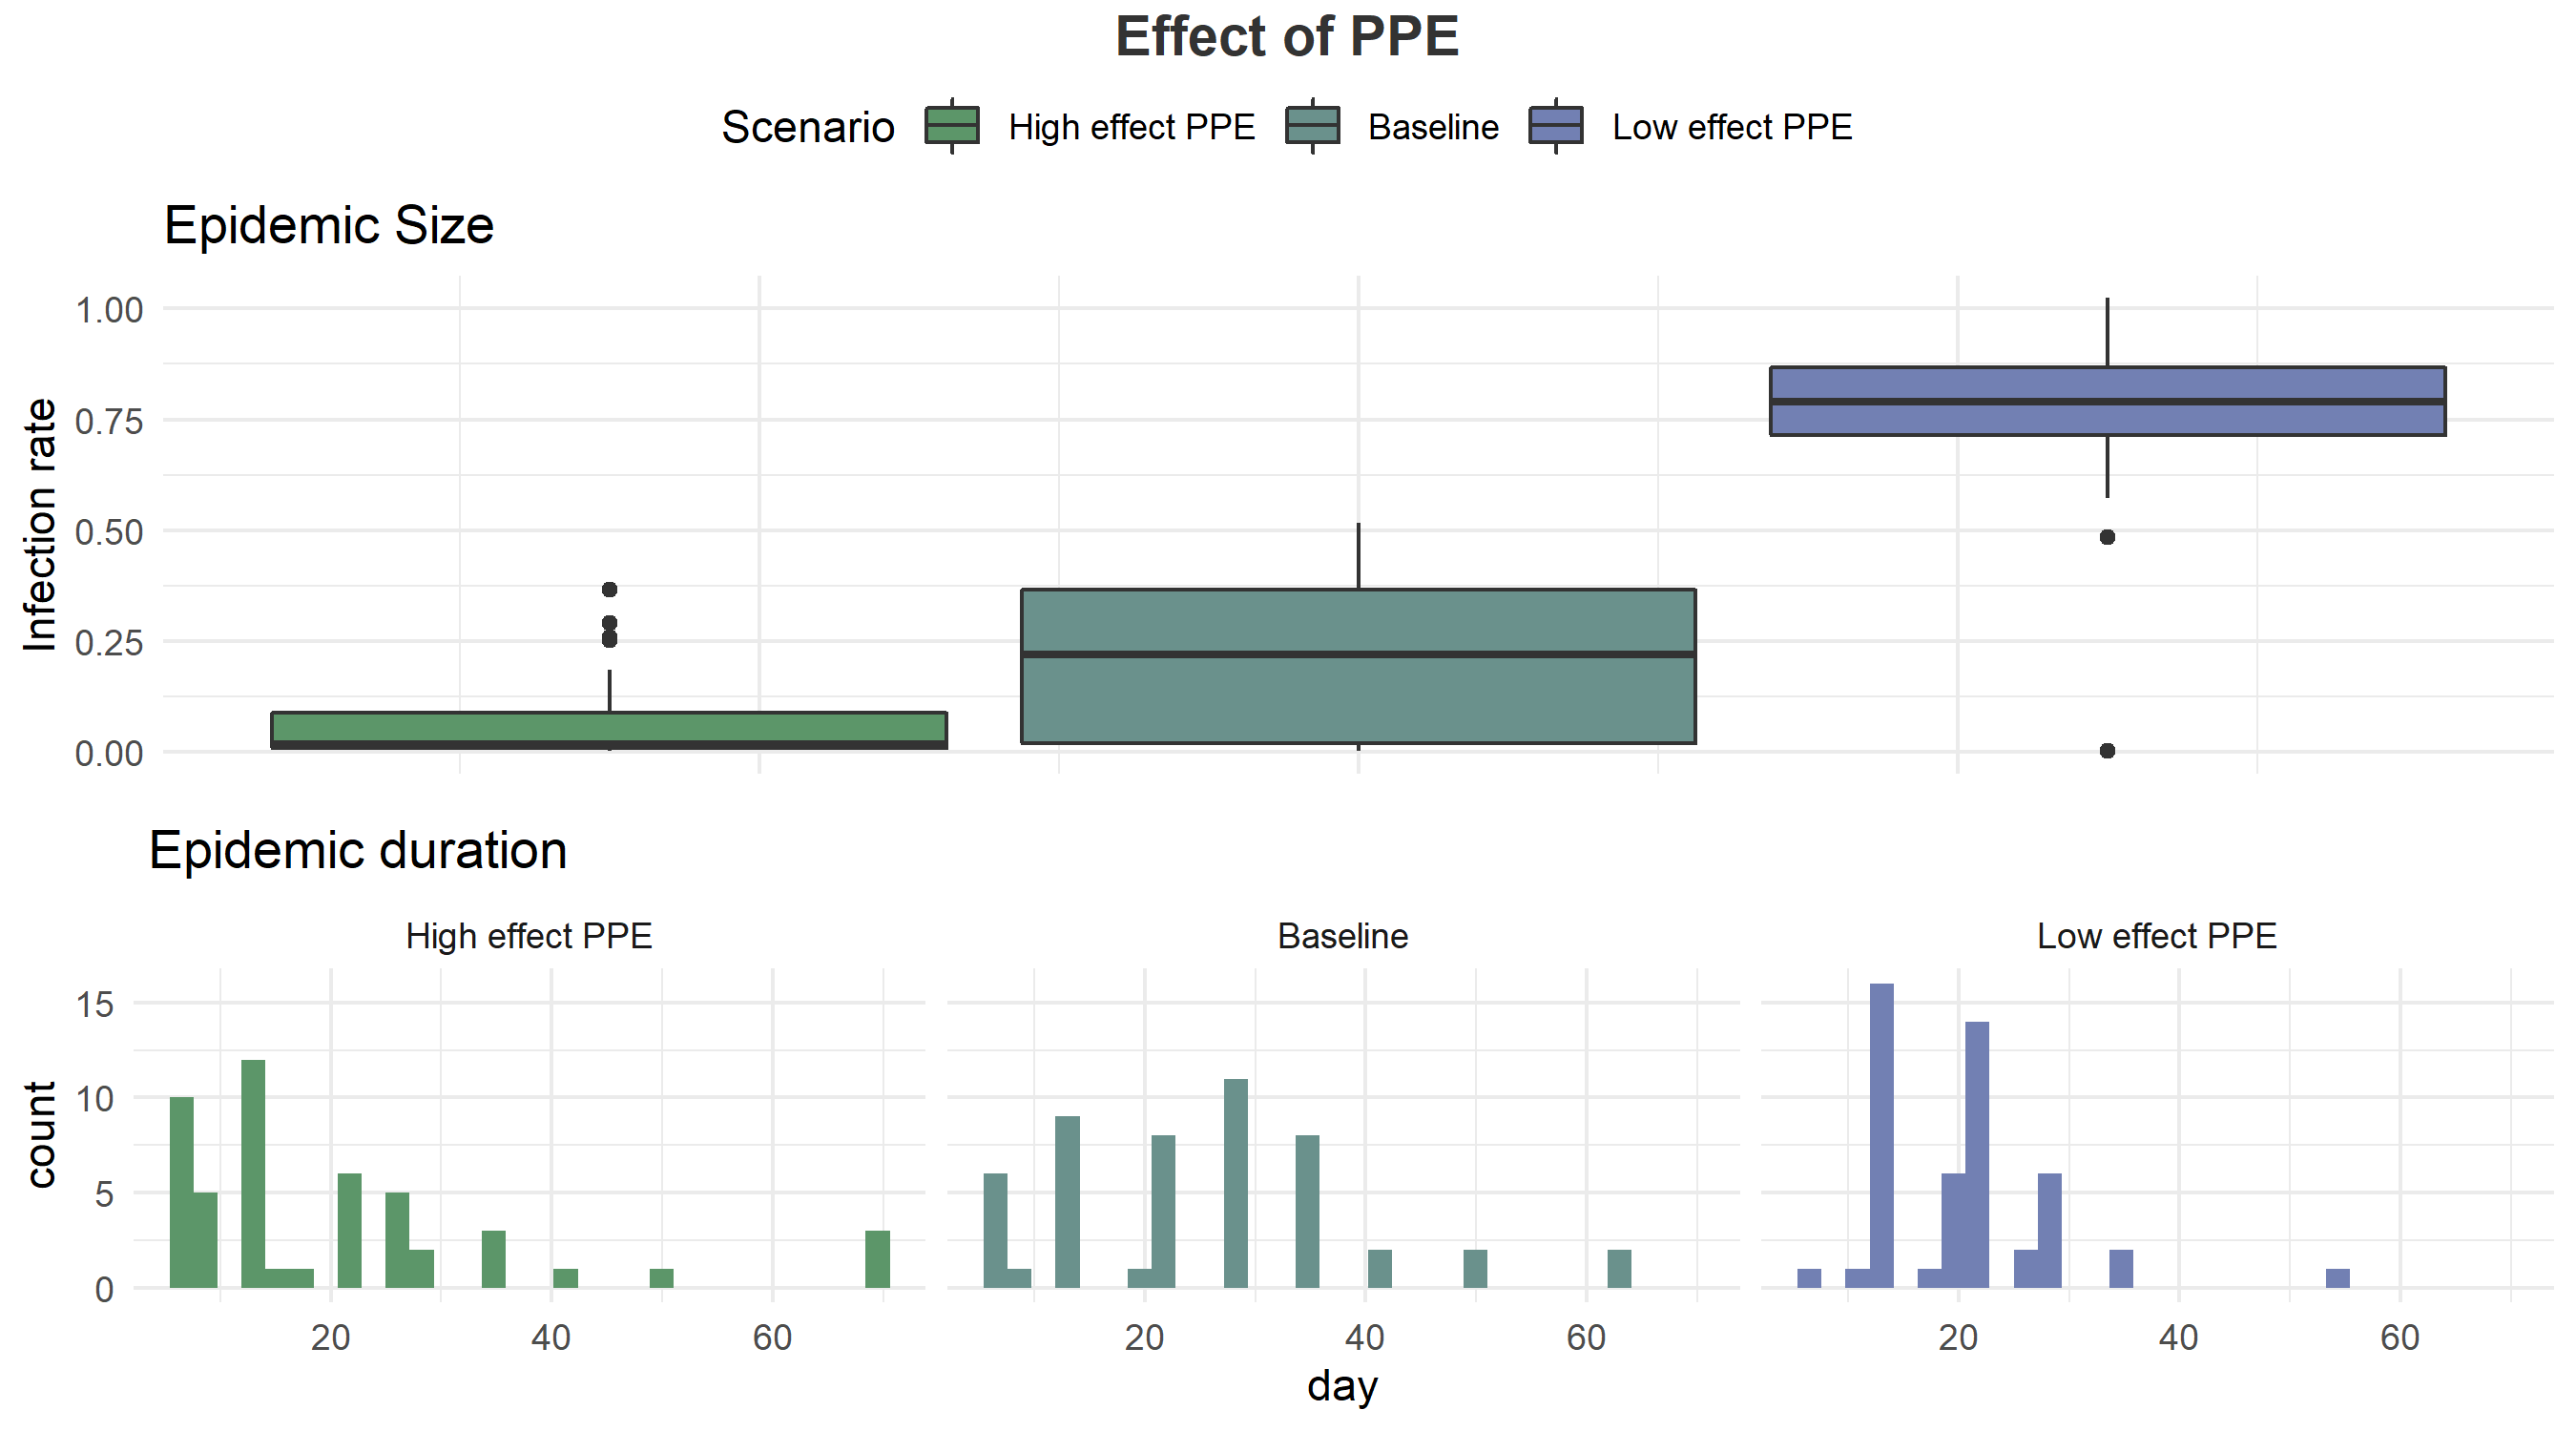
\includegraphics{Figures/SensitivityAnalysis/PPE}  
\end{figure}

\begin{figure}
\caption{Sensitivity analysis on the testing frequency}
\centering
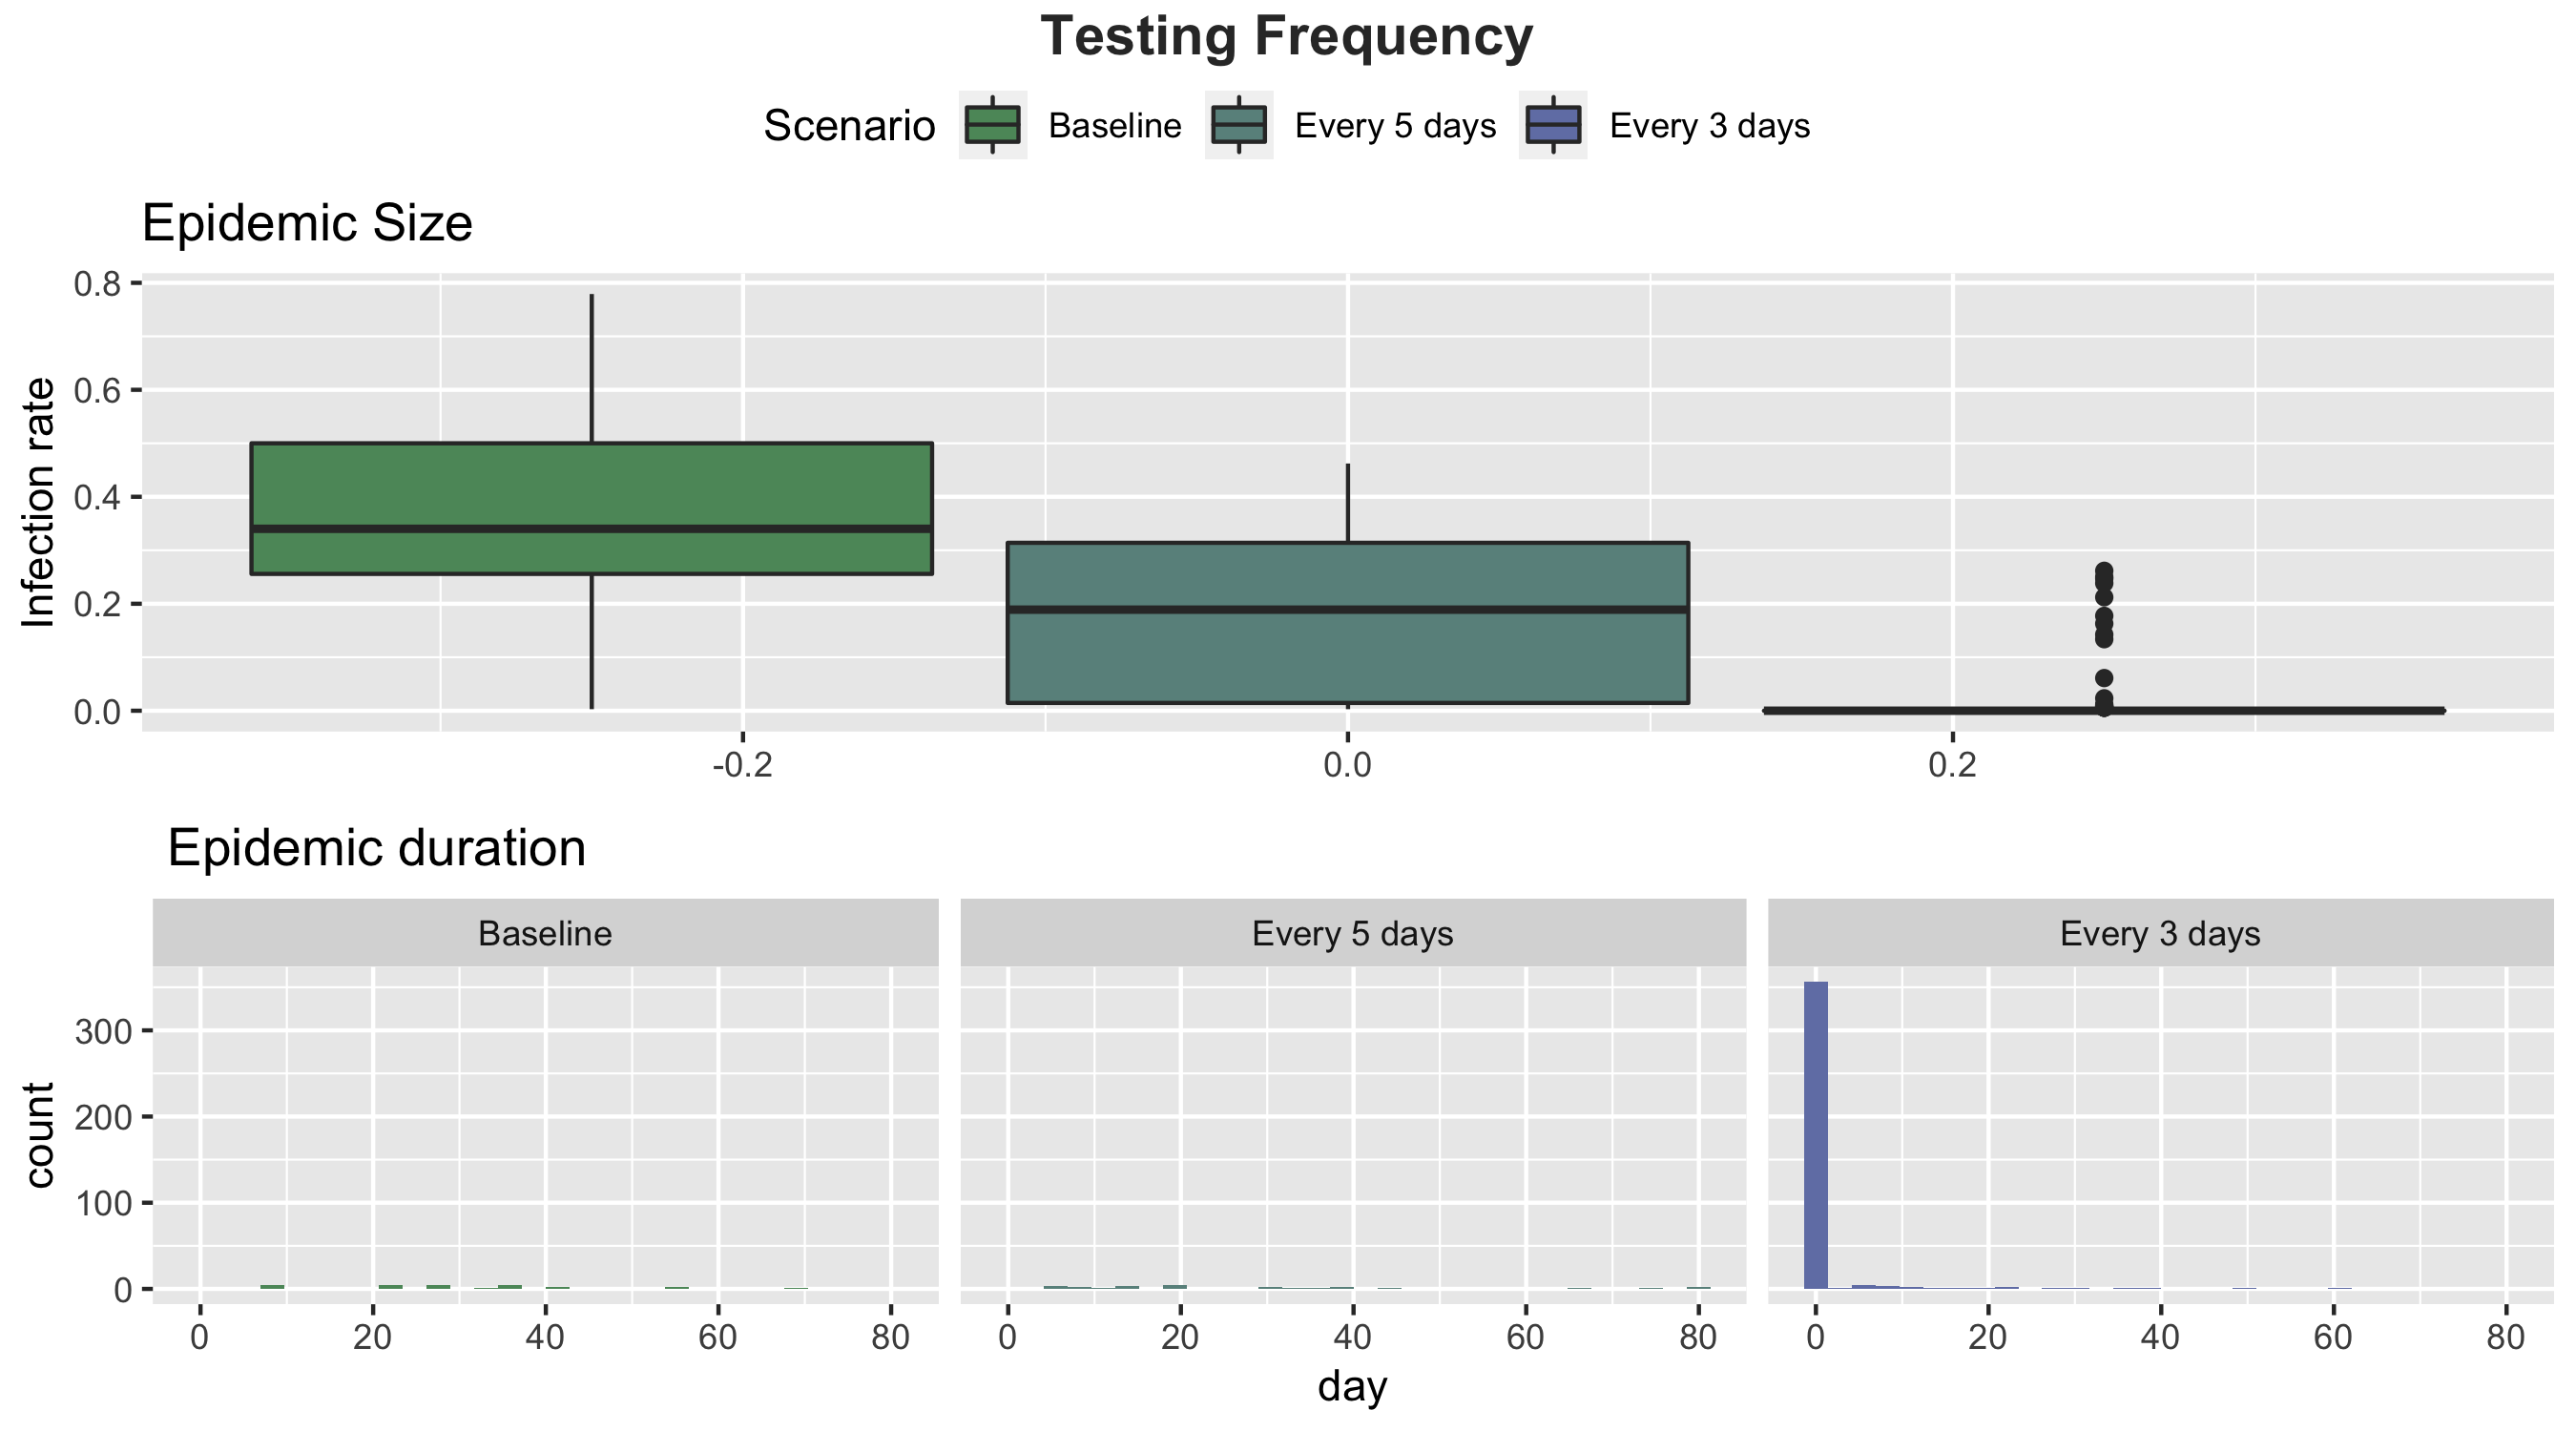
\includegraphics{Figures/SensitivityAnalysis/TestingFreq}
\end{figure}

\begin{figure}
\caption{Sensitivity analysis on the effect of vaccination}
\centering
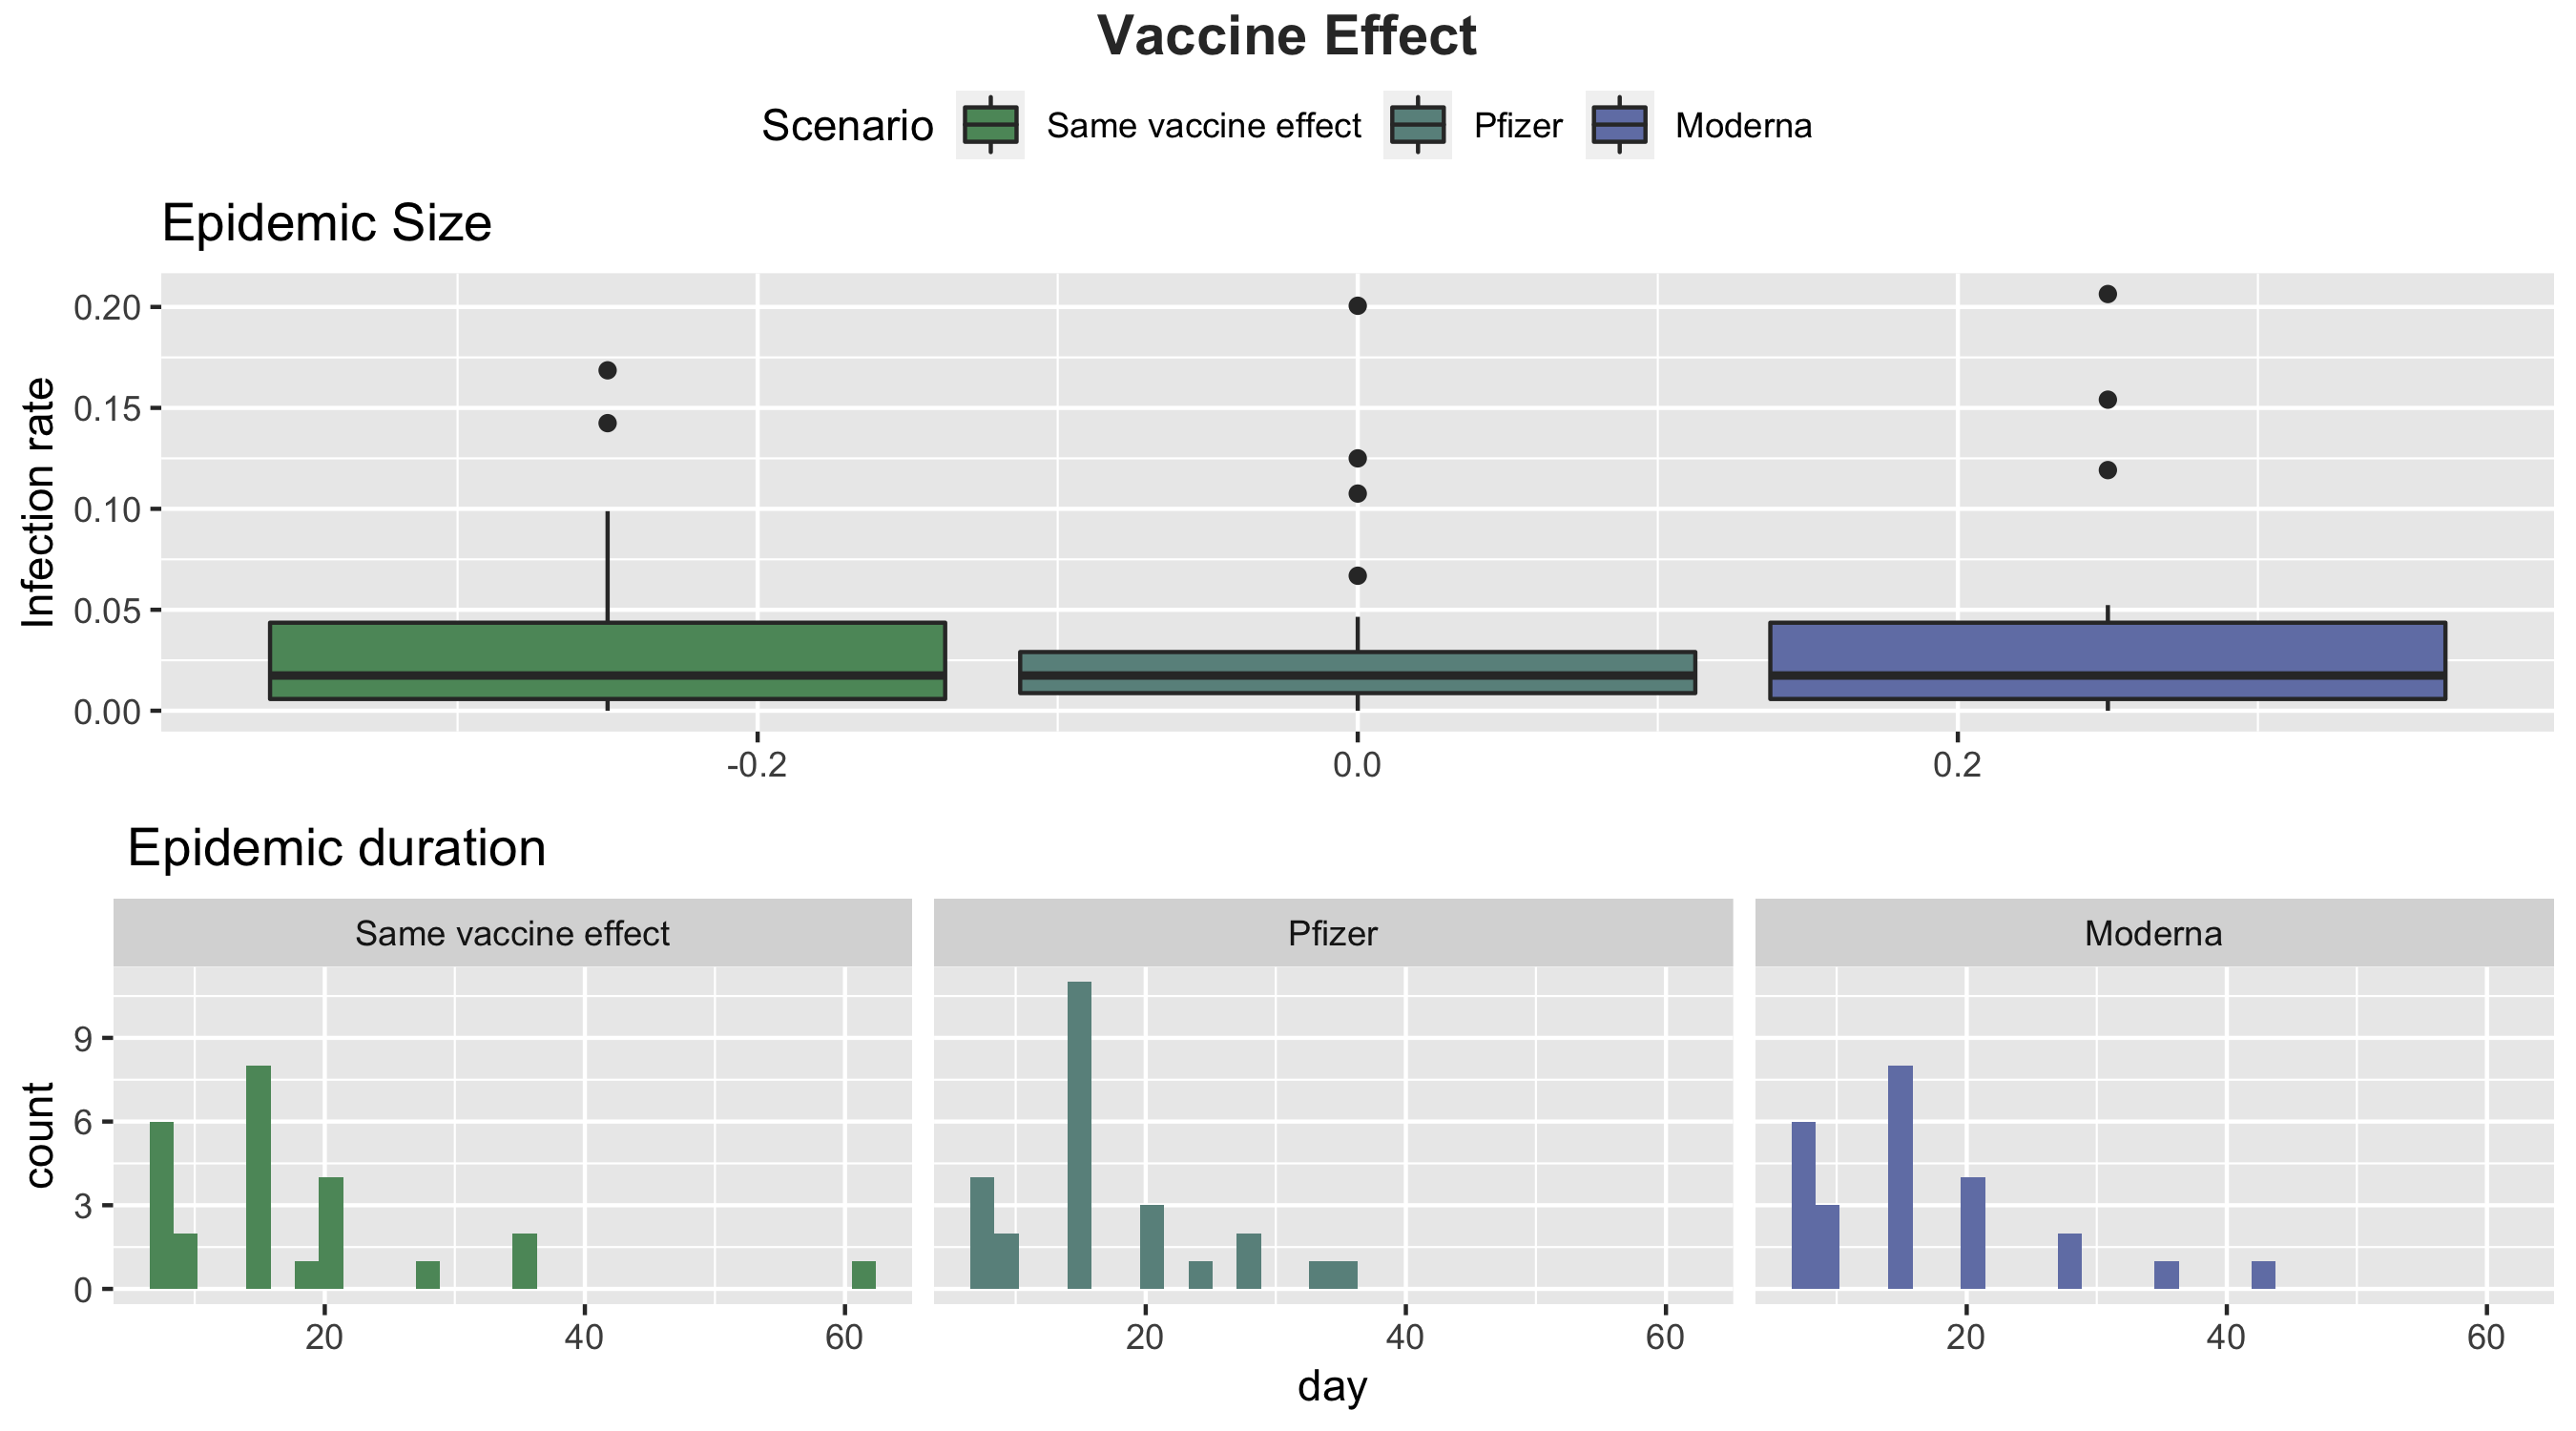
\includegraphics{Figures/SensitivityAnalysis/VaccinationEf}  
\end{figure}

\hypertarget{scenario-modeling-1}{%
\subsection{Scenario modeling}\label{scenario-modeling-1}}

\begin{figure}
\caption{Scenario with lowe ccommunity transmission}
\centering
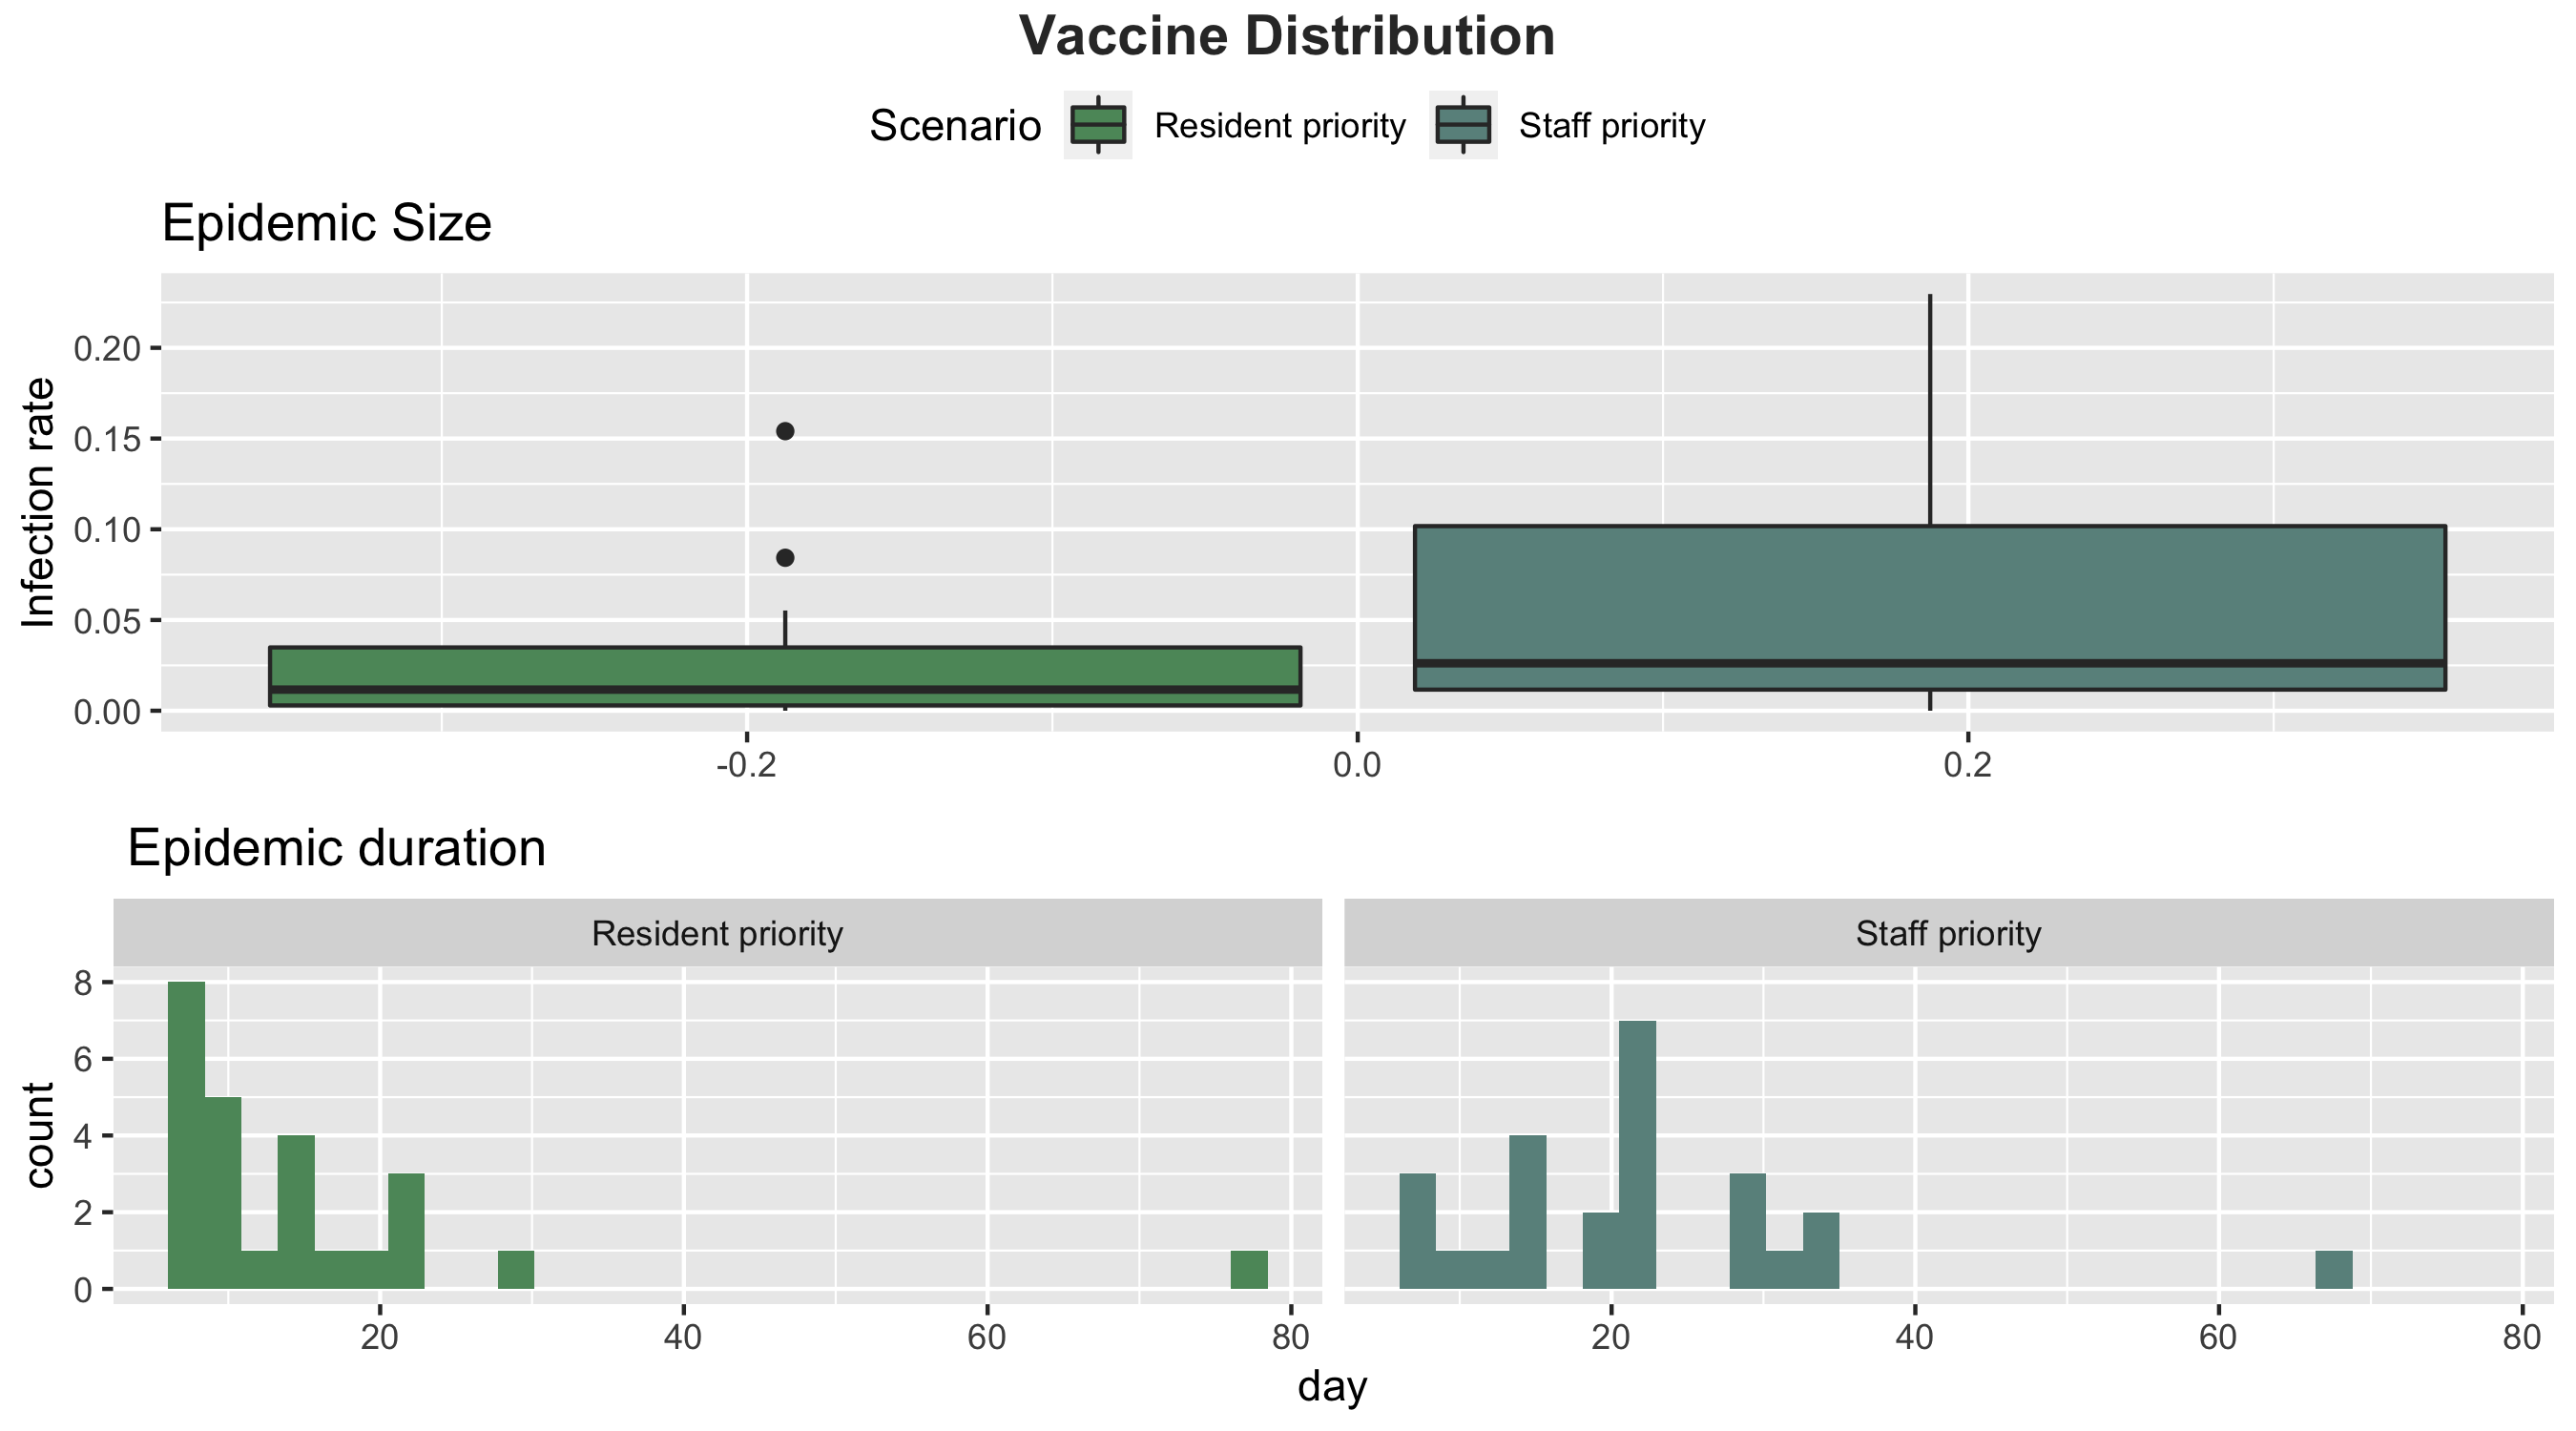
\includegraphics{Figures/Scenarios/VaccineDist}
\end{figure}

\hypertarget{references}{%
\section*{References}\label{references}}
\addcontentsline{toc}{section}{References}

\hypertarget{refs}{}
\begin{cslreferences}
\leavevmode\hypertarget{ref-Baden2020}{}%
Baden, Lindsey R., Hana M. El Sahly, Brandon Essink, Karen Kotloff,
Sharon Frey, Rick Novak, David Diemert, et al. 2020. ``Efficacy and
Safety of the mRNA-1273 SARS-CoV-2 Vaccine.'' \emph{New England Journal
of Medicine}, December, NEJMoa2035389.
\url{https://doi.org/10.1056/NEJMoa2035389}.

\leavevmode\hypertarget{ref-Chu2020}{}%
Chu, Derek K., Elie A. Akl, Stephanie Duda, Karla Solo, Sally Yaacoub,
Holger J. Schünemann, Amena El-harakeh, et al. 2020. ``Physical
distancing, face masks, and eye protection to prevent person-to-person
transmission of SARS-CoV-2 and COVID-19: a systematic review and
meta-analysis.'' \emph{The Lancet} 395 (10242): 1973--87.
\url{https://doi.org/10.1016/S0140-6736(20)31142-9}.

\leavevmode\hypertarget{ref-He2020}{}%
He, Xi, Eric H. Y. Lau, Peng Wu, Xilong Deng, Jian Wang, Xinxin Hao, Yiu
Chung Lau, et al. 2020. ``Temporal dynamics in viral shedding and
transmissibility of COVID-19.'' \emph{Nature Medicine} 26 (5): 672--75.
\url{https://doi.org/10.1038/s41591-020-0869-5}.

\leavevmode\hypertarget{ref-Pfizer2020}{}%
Pfizer-BioNTech. 2020. ``Vaccines and Related Biological Products
Advisory Committee Meeting December 10, 2020.'' Pfizer-BioNTech.

\leavevmode\hypertarget{ref-Polack2020}{}%
Polack, Fernando P, Stephen J Thomas, Nicholas Kitchin, Judith Absalon,
Alejandra Gurtman, Stephen Lockhart, John L Perez, et al. 2020. ``Safety
and Efficacy of the BNT162b2 mRNA Covid-19 Vaccine.'' \emph{The New
England Journal of Medicine}, 2603--15.
\url{https://doi.org/10.1056/NEJMoa2034577}.
\end{cslreferences}

\end{document}
